\documentclass{article}
\usepackage{SDUstyle}
\sloppy

\fancyhf{}
\fancyhead[L]{
    \begin{minipage}[c]{0.2\textwidth}
        
\includegraphics[height=11mm]{imgs/logo.png}  %用于设置页眉左侧的图片
    \end{minipage}
}
\fancyhead[C]{端侧轻量级人脸检测模型对比研究与性能评估}     %用于设置页眉中间的文字
\setlength{\headheight}{32pt}

\fancyfoot[C]{\thepage}
% 设置页眉宽度为文本宽度
\setlength{\headwidth}{\textwidth}
% 设置页眉左侧偏移量,使其水平居中
\fancyhfoffset[L]{\dimexpr0.5\textwidth-0.5\textwidth\relax}

% 设置超链接颜色
\hypersetup{
    colorlinks=true,
    linkcolor=blue, % 超链接的颜色
    urlcolor=red,   % URL 的颜色
    citecolor=green % 引用的颜色
}


\begin{document}
\pagenumbering{Roman}
\setcounter{page}{0}

\begin{titlepage}
    \centering
    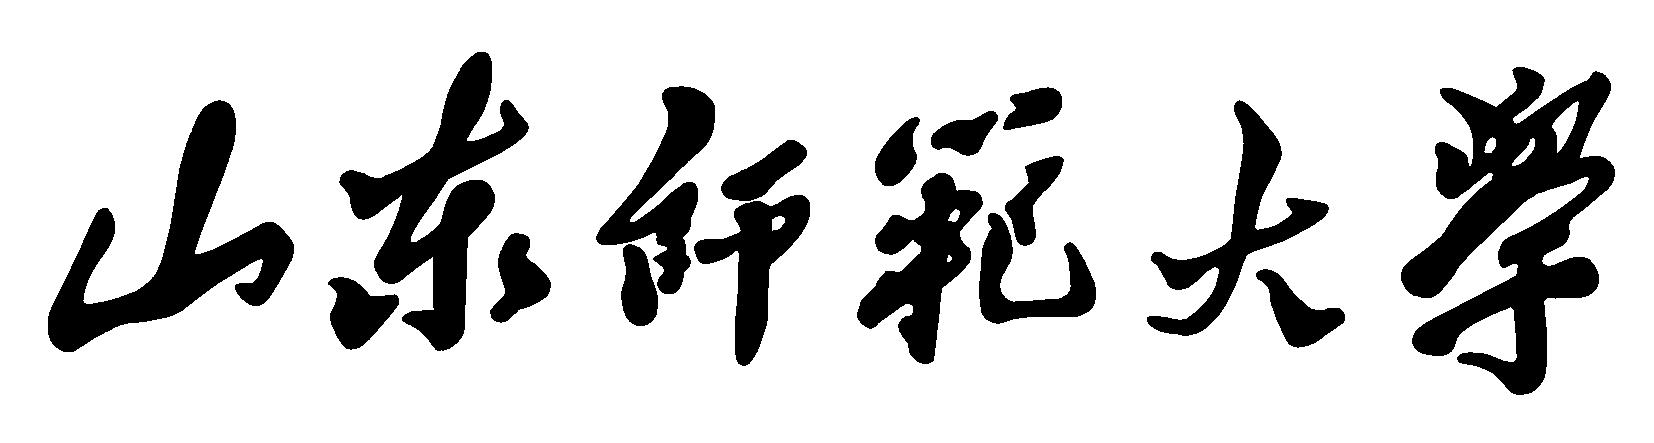
\includegraphics[width=0.65\textwidth]{./imgs/logo_text.png}
    \par\vspace{1.5cm}
    {\Huge \heiti 端侧轻量级人脸检测模型对比研究与性能评估 \par}
    \vspace{1cm}
    {\Large \heiti 《计算机视觉》Final Project \par}
    \vspace{5cm}

    \begin{center}
        {\Large
        \makebox[4em][s]{\heiti 姓名:}\underline{\makebox[15em][c]{\heiti 董霁兴}}\\
        \makebox[4em][s]{\heiti 学号:}\underline{\makebox[15em][c]{\heiti 2024317181}}\\
        \makebox[4em][s]{\heiti 班级:}\underline{\makebox[15em][c]{\heiti 计算机技术2班}}\\
        \makebox[4em][s]{\heiti 学院:}\underline{\makebox[15em][c]{\heiti 信息科学与工程学院}}\\
        }
    \end{center}

    \vfill
    {\Large \today} % 日期
\end{titlepage}
\setcounter{page}{1}    % 将页码计数器重置为1,使正文从第1页开始计数
\thispagestyle{empty}   % 将当前页面样式设置为空,即不显示页眉页脚和页码

\sectionfont{\centering}
\clearpage
\newpage

\setcounter{page}{1}
\section*{摘要}
\addcontentsline{toc}{section}{摘要 Abstract}   %用来目录中添加相应的条目
随着人工智能技术在移动设备和物联网领域的广泛应用,端侧人脸检测的需求日益增长。本文对当前主流的轻量级人脸检测模型进行了系统的对比研究。首先介绍了SqueezeNet、MobileNet和ShuffleNet等轻量化卷积神经网络的基本原理,随后重点分析了RetinaFace、BlazeFace和YOLO5Face三类代表性人脸检测模型的特点。实验中,我们将这些模型统一转换为ONNX格式,使用ONNX Runtime进行推理,并在WIDER FACE数据集和自建的单人人脸数据集上进行了全面评估。实验结果表明:RetinaFace和YOLO5Face系列在检测精度上具有优势,BlazeFace系列则在速度和模型大小方面表现突出,而YOLOv5n-0.5在各项性能指标上较为均衡。基于实验结果,本文针对不同应用场景提出了具体的模型选择建议,为端侧人脸检测的实际应用提供了重要参考。

\section*{Abstract}
With the widespread application of artificial intelligence technology in mobile devices and IoT, the demand for edge-side face detection has been growing rapidly. This paper presents a systematic comparative study of current mainstream lightweight face detection models. We first introduce the basic principles of lightweight convolutional neural networks including SqueezeNet, MobileNet, and ShuffleNet, followed by a detailed analysis of three representative face detection models: RetinaFace, BlazeFace, and YOLO5Face. In our experiments, these models were uniformly converted to ONNX format and inferenced using ONNX Runtime, with comprehensive evaluations conducted on both the WIDER FACE dataset and our self-built single-face dataset. The results demonstrate that RetinaFace and YOLO5Face series excel in detection accuracy, while BlazeFace series shows advantages in speed and model size, and YOLOv5n-0.5 achieves a balanced performance across all metrics. Based on these findings, we provide specific model selection recommendations for different application scenarios, offering valuable reference for practical implementation of edge-side face detection.

\vfill % 用于在垂直方向上填充剩余空间,使内容均匀分布

% \clearpage 命令用于:
% 1. 将所有未处理的浮动体(如图表)强制输出到当前页
% 2. 结束当前页并开始新的一页
% 3. 清除当前页面的所有内容
\clearpage

\addcontentsline{toc}{section}{目录 Table of Contents}
\thispagestyle{empty}
\hypersetup{linkcolor=black}
\tableofcontents
\hypersetup{linkcolor=blue}
\newpage


\setcounter{page}{1}
\pagenumbering{arabic}

\section{引言}
\subsection{研究背景}
人脸检测技术在当今社会有着广泛的应用价值,是人脸智能分析应用的核心基础组件。它为人脸识别、人脸属性分析(如年龄估计、性别识别、颜值打分和表情识别)、表情识别、智能视频监控、人脸图像过滤、智能图像裁切、人脸 AR 等众多应用提供了基础支持。例如,在智能安防领域,人脸检测可以快速识别监控画面中的人脸,为后续的分析和处理提供关键信息;在社交娱乐应用中,人脸检测可以实现有趣的特效和互动功能。

需要特别说明的是,人脸检测和人脸识别是两个不同的任务。人脸检测主要是在图像或视频中检测出人脸所在的位置和边界框,其目标是确定图像中是否存在人脸,并标识出其大致位置,它通常作为更高级别任务(如人脸识别、表情识别等)的预处理步骤。而人脸识别则是指识别和验证人脸的身份,目标是将输入的人脸图像与预先存储的人脸模板进行比较,并判断是否匹配。

随着移动设备和物联网的快速发展,端侧人脸检测的需求日益增长。然而,端侧设备通常面临着计算资源有限、存储空间受限、功耗要求严格等约束。因此,如何在保证检测精度的同时,实现模型的轻量化和高效推理,成为了当前研究的重要方向。

\subsection{技术发展历程}
到目前为止,人脸检测技术的发展经历了两个主要阶段:基于手工特征的传统方法和基于深度学习的方法。

基于手工特征的传统方法主要依赖于手工设计的特征,早期方法可分为四大类\cite{yang2002detecting}:基于知识的方法、特征不变方法、模板匹配方法和基于外观的方法。例如,基于知识的方法利用人类对典型面孔结构的先验知识,通过提取面部特征并根据编码规则区别候选人脸;特征不变方法寻找对姿态和光照变化具有鲁棒性的人脸结构特征;模板匹配方法使用预先存储的人脸模板来确定人脸位置,但在处理尺寸、姿势和形状变化等问题上存在不足;基于外观的方法从训练人脸图像中学习人脸模型。

随着深度学习技术的发展,基于深度学习的人脸检测方法逐渐成为研究主流。这类方法能够自动学习图像中的复杂特征,在检测准确率上取得了显著优势。其架构主要分为多阶段检测架构、两阶段检测架构和单阶段检测架构\cite{feng2021detect}。在端侧场景下,单阶段检测架构(如SSD、RetinaNet)因其较好的速度和精度平衡,成为了主流选择。同时,为了适应端侧设备的资源限制,各种轻量化网络结构(如MobileNet、ShuffleNet等)被广泛应用于人脸检测模型中,以降低计算复杂度和模型大小。

\subsection{端侧人脸检测的意义}
在实际应用中,端侧的轻量级人脸检测模型具有至关重要的意义。端侧设备,如手机端、嵌入式设备和开发板设备,资源有限,包括计算能力、存储容量和功耗等方面。端侧的轻量级人脸检测模型能够在这些资源受限的设备上高效运行,实现实时的人脸检测功能。

在手机端,轻量级人脸检测模型可以应用于自拍美颜、视频通话中的人脸跟踪自动对焦等功能。在嵌入式设备和开发板设备方面,如智能安防摄像头、智能门禁系统等,轻量级人脸检测模型可以在低功耗的情况下,快速准确地检测人脸,实现对人员的实时监控和身份识别,为保障公共安全和企业管理提供了有力支持。

此外,端侧推理相比云端推理具有隐私保护、低延迟、低带宽占用等优势。在某些对隐私要求较高或网络条件不稳定的场景下,端侧人脸检测成为了必然选择。

本研究的主要目标是通过系统性的分析和实验评估,为端侧人脸检测模型的选择和应用提供理论与实践指导。具体而言,研究工作包含两个主要方面:首先,对人脸检测任务的技术演进、轻量化卷积神经网络的核心原理以及端侧人脸检测模型的最新研究进展进行全面综述,系统梳理相关领域的理论基础和技术发展脉络;其次,针对当前主流的轻量级人脸检测模型,构建标准化的测试框架,在统一的软硬件环境下进行全面的性能评估,通过定量分析模型在检测精度、推理速度和资源占用等维度的表现,结合不同应用场景的具体需求,提出有针对性的模型选择建议,为端侧人脸检测的工程实践提供可靠的决策依据。

\clearpage

\section{轻量化卷积网络}

在端侧轻量级人脸检测模型,特别是单阶段检测架构中,backbone 的选择起着关键作用。它负责提取图像的特征,其性能和效果直接影响整个模型的效率和准确性。目前主流端侧模型都会优先考虑使用轻量化架构作为 backbone。本节将详细介绍三个经典的轻量化卷积网络:SqueezeNet、MobileNet 和 ShuffleNet。需要特别说明的是,这些网络都迭代了多个版本,本文仅对各个轻量化卷积网络模型的初始版本做介绍。

\subsection{SqueezeNet}
SqueezeNet\cite{iandola2016squeezenet} 于 2016 年 2 月由伯克利和斯坦福研究人员首次发表在 arxiv 上。它是较早提出的一个轻量化神经网络,能够在保持和 AlexNet 相同准确率的情况下,将模型参数减少到原来的 50 倍。在通过 Deep Compression 压缩后,可以将模型压缩至 0.47MB。这种高效的压缩比使其特别适合在资源受限的端侧设备上部署。

SqueezeNet 提出了三个核心的架构设计策略来减小 CNN 模型参数量:
\begin{enumerate}
    \item 用 1$\times$1 卷积替代 3$\times$3 卷积:由于 1$\times$1 卷积的参数量仅为 3$\times$3 卷积的 1/9,这种替换可以显著减少模型参数
    \item 减少 3$\times$3 卷积的输入通道数:通过在 3$\times$3 卷积层之前使用 squeeze 层来减少输入通道数,从而降低参数量
    \item 延迟下采样,使卷积层保持较大的特征图尺寸:这种策略通过在网络后期才进行降采样,使得卷积层能够在较大的特征图上工作,从而提取更多的特征信息
\end{enumerate}

其中,第一、第二条策略主要用于减小模型的参数量和计算复杂度,而第三条策略则是为了在模型压缩的同时保持较高的准确率。这种权衡反映了模型设计中精度与效率的折中考虑。

\begin{figure}[htbp]
    \centering
    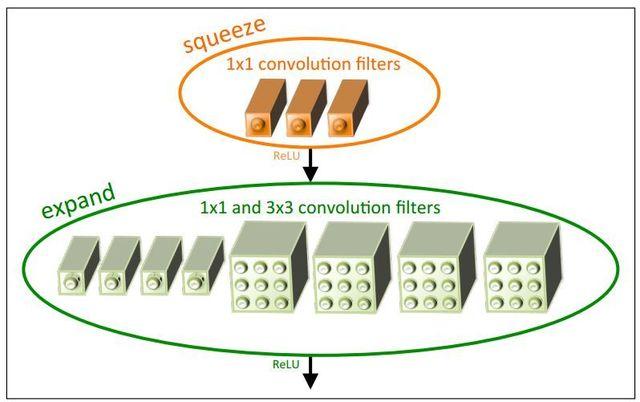
\includegraphics[width=0.7\linewidth]{imgs/fire_module.jpg}
    \caption{Fire Module 结构}
    \label{fig:fire_module}
\end{figure}

SqueezeNet 的核心创新在于提出了 Fire Module 结构,如图 \ref{fig:fire_module} 所示。Fire Module 由 squeeze 层和 expand 层两个关键组件构成:
\begin{itemize}
    \item squeeze 层:使用 1$\times$1 卷积对输入特征图进行通道数压缩,起到降维作用
    \item expand 层:包含平行的 1$\times$1 和 3$\times$3 卷积分支,并将其输出在通道维度上拼接。这种设计既保持了模型的特征提取能力,又控制了参数量的增长
\end{itemize}

Fire Module 的设计体现了"多分支+通道重组"的思想,这一思想后来被广泛应用于各类轻量级网络中。通过堆叠多个 Fire Module,SqueezeNet 形成了一个深层但参数量小的网络结构。

\begin{figure}[htbp]
    \centering
    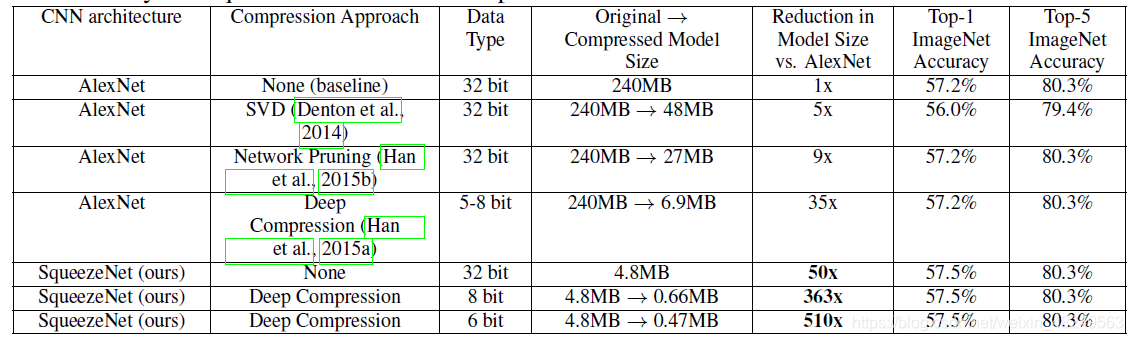
\includegraphics[width=0.8\linewidth]{imgs/squeezenet_vs_alexnet.png}
    \caption{SqueezeNet 与 AlexNet 在 ImageNet 上的性能对比}
    \label{fig:squeezenet_comp}
\end{figure}

如图 \ref{fig:squeezenet_comp} 所示,在 ImageNet 数据集上的实验结果表明,SqueezeNet 在 TOP-1 和 TOP-5 准确率上与 AlexNet 相当,但模型参数量仅为 AlexNet 的 1/50。这一突破性成果证明了轻量化网络设计的可行性,为后续轻量级网络的发展奠定了重要基础。值得注意的是,SqueezeNet 虽然在参数压缩方面取得了显著成果,但其推理速度相比于后来的 MobileNet 等网络仍有提升空间,这也促使了后续更多轻量级网络的研究与发展。

\subsection{MobileNet}
MobileNet\cite{howard2017mobilenets} 由 Google 团队于 2017 年 4 月提出,是一种专门为移动和嵌入式设备设计的高效深度神经网络架构。其核心创新在于提出深度可分离卷积(Depthwise Separable Convolution)操作,通过分解标准卷积运算显著降低了模型的计算复杂度和参数量。这种设计不仅保持了良好的特征提取能力,还使得模型能够在资源受限的端侧设备上高效运行。

\begin{figure}[htbp]
    \centering
    \begin{subfigure}[b]{0.32\textwidth}
        \centering
        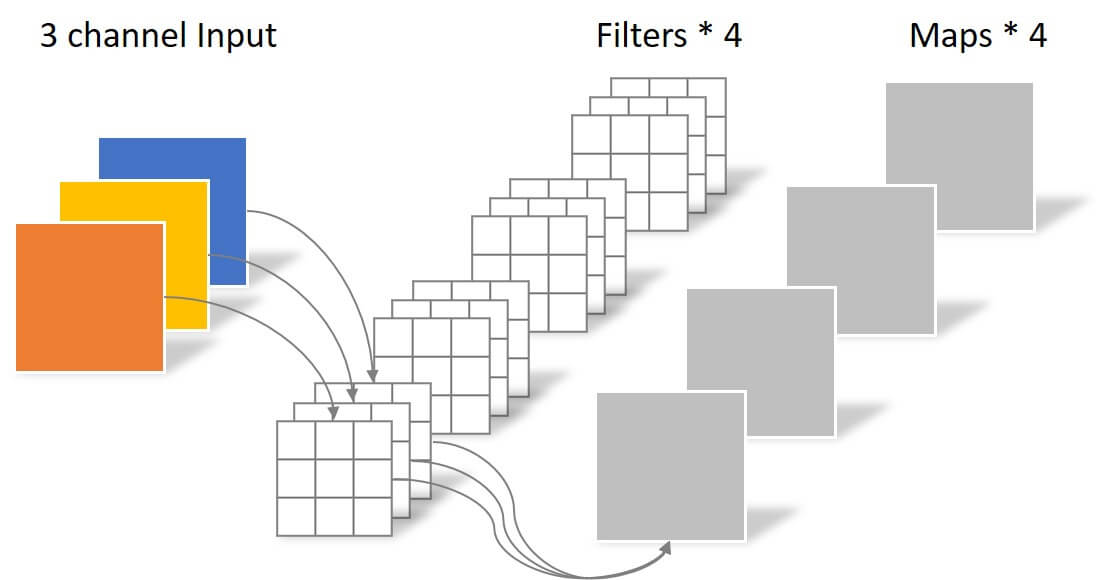
\includegraphics[width=\linewidth]{imgs/std_cov.jpg}
        \caption{标准卷积}
    \end{subfigure}
    \begin{subfigure}[b]{0.32\textwidth}
        \centering
        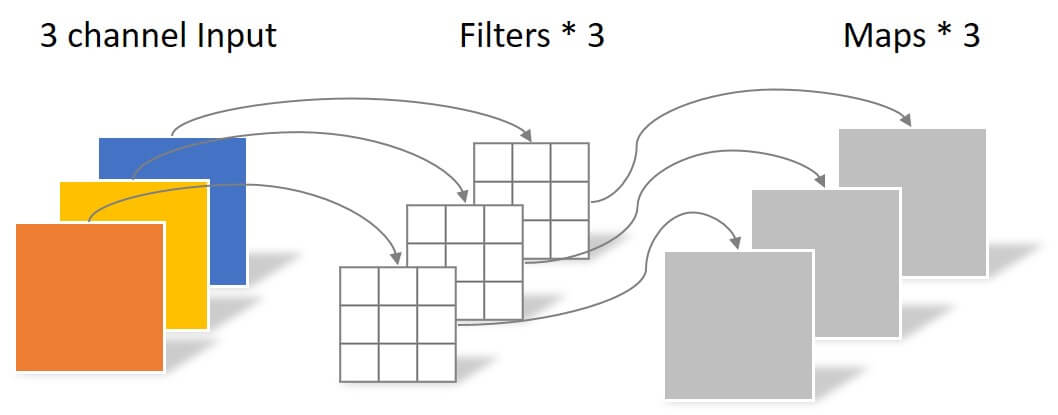
\includegraphics[width=\linewidth]{imgs/dpth_cov.jpg}
        \caption{深度卷积}
    \end{subfigure}
    \begin{subfigure}[b]{0.32\textwidth}
        \centering
        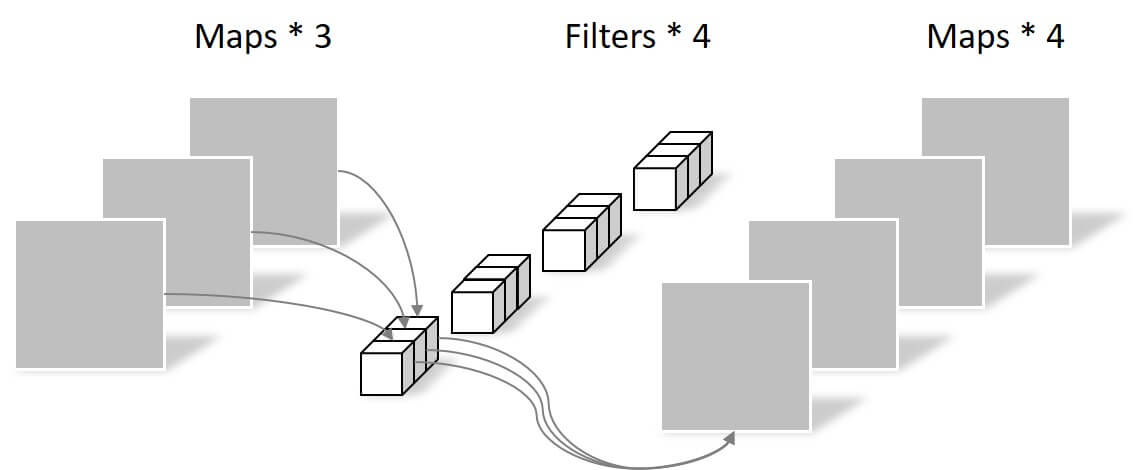
\includegraphics[width=\linewidth]{imgs/sep_cov.jpg}
        \caption{逐点卷积}
    \end{subfigure}
    \caption{深度可分离卷积示意图}
    \label{fig:mobilenet_conv}
\end{figure}

如图 \ref{fig:mobilenet_conv} 所示,深度可分离卷积将标准卷积分解为两个独立的操作:
\begin{itemize}
    \item 深度卷积(Depthwise Convolution):对输入特征图的每个通道独立应用空间卷积,实现空间维度上的特征提取。这一步骤保留了局部空间相关性。
    \item 逐点卷积(Pointwise Convolution):使用 1$\times$1 卷积对深度卷积的输出进行通道维度的特征融合,确保输出特征图能够包含所有输入通道的信息。这一步骤建立了跨通道的相关性。
\end{itemize}

为了定量分析深度可分离卷积带来的计算效率提升,我们对其参数量和计算量进行理论分析。假设输入特征图尺寸为 $D_F \times D_F \times M$,输出特征图通道数为 $N$,卷积核大小为 $D_K \times D_K$。那么:

标准卷积的计算量为:
\begin{equation}
    D_K \cdot D_K \cdot M \cdot N \cdot D_F \cdot D_F
\end{equation}

深度可分离卷积的计算量为:
\begin{equation}
    D_K \cdot D_K \cdot M \cdot D_F \cdot D_F + M \cdot N \cdot D_F \cdot D_F
\end{equation}

两者的计算量比值为:
\begin{equation}
    \frac{1}{N} + \frac{1}{D_K^2}
\end{equation}

对于典型的 $3\times3$ 卷积核,当输出通道数 $N$ 较大时,深度可分离卷积可以将计算量降低到标准卷积的约 $\frac{1}{8}$ 到 $\frac{1}{9}$。

MobileNet 的网络架构由一系列深度可分离卷积块堆叠而成,每个块包含一个深度卷积层和一个逐点卷积层,并在深度卷积后使用 BatchNorm 和 ReLU 非线性激活函数。此外,MobileNet 还引入了两个重要的超参数:
\begin{itemize}
    \item 宽度乘子 $\alpha$:用于控制每层的通道数,从而调节模型容量
    \item 分辨率乘子 $\rho$:用于控制输入图像分辨率,影响特征图大小
\end{itemize}

\begin{figure}[htbp]
    \centering
    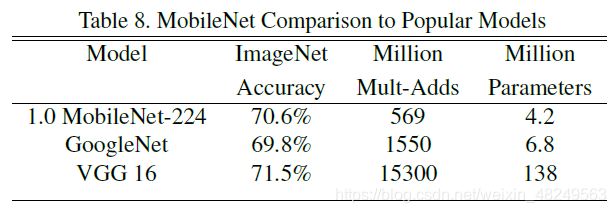
\includegraphics[width=0.8\linewidth]{imgs/mobilenet_comp.png}
    \caption{MobileNet 与其他模型在 ImageNet 上的性能对比}
    \label{fig:mobilenet_comp}
\end{figure}

如图 \ref{fig:mobilenet_comp} 所示,在 ImageNet 分类任务上,标准 MobileNet($\alpha=1$)达到了 70.6\% 的 TOP-1 准确率,超过了 GoogLeNet(69.8\%),但模型大小仅为 4.2MB,推理时间约为 GoogLeNet 的三分之一。相比 VGG-16,虽然准确率略低 0.9 个百分点,但参数量减少了 32 倍,计算量减少了 27 倍。这些实验结果充分证明了 MobileNet 在模型效率和准确性之间取得了优秀的平衡。

\subsection{ShuffleNet}
ShuffleNet\cite{zhang2018shufflenet} 是由 Face++ 团队(旷世科技)于 2017 年提出的一种高效的卷积神经网络架构。通过对 MobileNet 的深入分析,研究团队发现其中的 1$\times$1 逐点卷积占用了大量计算资源(约 94.8\% 的计算量),这严重制约了模型在资源受限设备上的部署。为解决这一问题,ShuffleNet 提出了两个创新性的架构设计:逐点分组卷积(Pointwise Group Convolution)和通道重排(Channel Shuffle)。

逐点分组卷积通过将输入特征图的通道分成若干组,每组独立进行 1$\times$1 卷积运算,显著降低了计算复杂度。具体而言,若将通道分为 g 组,计算量可降低至原来的 1/g。然而,分组卷积会导致不同组之间的特征信息无法直接交互,限制了模型的表达能力。为克服这一局限性,ShuffleNet 创新性地引入了通道重排操作,通过系统性地重新排列特征通道,实现了不同组之间的信息流动,在保持低计算复杂度的同时提高了特征的表达能力。

ShuffleNet 的核心单元由以下三个部分组成:
\begin{itemize}
    \item 第一个逐点分组卷积层,负责降低特征通道数,减少计算量
    \item 通道重排操作,促进不同组之间的信息交换
    \item 深度可分离卷积和第二个逐点分组卷积层,进一步提取和融合特征
\end{itemize}

此外,ShuffleNet 还采用了残差连接结构,并在网络不同阶段通过步长为 2 的卷积实现特征图尺寸的降采样。为适应不同的计算资源约束,ShuffleNet 提供了一个宽度因子来调节网络规模。

\begin{figure}[htbp]
    \centering
    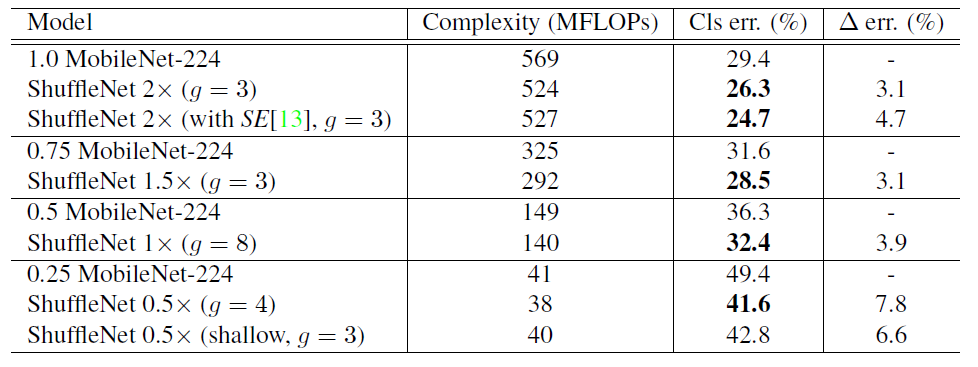
\includegraphics[width=0.8\linewidth]{imgs/shufflenet_comp.png}
    \caption{ShuffleNet 与其他模型在 ImageNet 上的性能对比}
    \label{fig:shufflenet_comp}
\end{figure}

如图 \ref{fig:shufflenet_comp} 所示,在相同参数量约束下,ShuffleNet 在 ImageNet 分类任务上的 TOP-1 准确率显著优于 MobileNet。具体而言,当模型参数量控制在 5M 以下时,ShuffleNet 比 MobileNet 实现了约 2-3 个百分点的准确率提升。这一结果充分证明了 ShuffleNet 在轻量级网络设计中的优越性,为后续移动端深度学习模型的发展提供了重要的架构参考。

\clearpage

\section{轻量级人脸检测模型}

在本研究中,我们选择了三个具有代表性的轻量级人脸检测模型进行实验和分析:RetinaFace、YOLO5Face 和 BlazeFace。这些模型的选择基于以下考虑:
\begin{itemize}
    \item 模型具有良好的轻量化特性和实时性能
    \item 在当前端侧轻量化模型实践中应用广泛
    \item 在 WiderFace 等标准数据集上取得了较好的排名
\end{itemize}

需要说明的是,除了本文选择的这三个模型外,YuNet、FaceBoxes、MogFace 等模型在实际应用中也有广泛使用,但考虑到实验规模和代表性,本研究仅对上述三个模型进行深入分析。

\subsection{RetinaFace}
RetinaFace\cite{deng2019retinaface} 是 Insight Face 团队在 2019 年提出的单阶段人脸检测模型,其在 WIDER FACE 数据集上取得了当时最先进的性能。该模型的主要创新点体现在以下几个方面:

\begin{enumerate}
    \item 多任务学习框架
    \begin{itemize}
        \item 提出了一种统一的多任务学习框架,将监督学习和自监督学习相结合
        \item 同时完成人脸检测、五个面部关键点定位和密集人脸 3D 回归预测
        \item 通过多任务学习增强了特征的表达能力,提高了模型的泛化性能
        \item 引入了自监督的网格像素回归分支,有效提升了对遮挡和极端姿态的鲁棒性
    \end{itemize}
    
    \item 特征金字塔网络改进
    \begin{itemize}
        \item 采用改进的特征金字塔结构(FPN)处理不同尺度的人脸,支持从 16$\times$16 到 512$\times$512 像素的人脸检测
        \item 引入了基于 deformable convolution 的上下文注意力机制,增强了特征提取能力
        \item 设计了自适应特征池化层,有效处理人脸变形和遮挡问题
        \item 在不同层级的特征图上共享检测头参数,减少了模型参数量
    \end{itemize}
    
    \item 灵活的 backbone 选择与损失函数设计
    \begin{itemize}
        \item 支持多种主干网络,包括 ResNet-50、ResNet-152、MobileNet 等
        \item 采用多任务联合损失函数,包括分类损失、边界框回归损失、关键点回归损失和密集回归损失
        \item 引入 focal loss 缓解正负样本不平衡问题
        \item 本实验选用 MobileNet-0.25 和 MobileNet v2 作为轻量级版本,以适应端侧部署需求
    \end{itemize}
\end{enumerate}

RetinaFace 采用了典型的单阶段检测器架构,但通过多任务学习和特征增强显著提升了检测性能。在 WIDER FACE 数据集的困难集上,RetinaFace-ResNet50 实现了 91.4\% 的 AP,创下了新的记录。在本次实验中,我们选用了其轻量级版本,具体包括:
\begin{itemize}
    \item RetinaFace-MobileNet0.25:使用 MobileNet-0.25 作为主干网络,模型大小仅 1.68MB,在 WIDER FACE 困难集上仍能达到 75.2\% 的 AP
    \item RetinaFace-MobileNetV2:采用 MobileNet v2 作为主干网络,在精度和速度上取得更好平衡,困难集 AP 达到 82.5\%
\end{itemize}

这些轻量级版本保留了原始 RetinaFace 的核心创新,同时通过网络压缩和量化优化实现了端侧友好的资源占用。它们可以直接对原始图片进行推理,无需预处理缩放,这一特性使其特别适合在计算资源受限的端侧设备上部署。

\subsection{BlazeFace}
BlazeFace\cite{bazarevsky2019blazeface} 是 Google Research 团队于 2019 年提出的一款专门针对移动 GPU 优化的轻量级人脸检测器,是目前 Google ML Kit 和 MediaPipe 框架的核心人脸检测组件。该模型在保持较高检测精度的同时,实现了超实时的性能表现,在移动设备上可达到 200-1000 FPS 的推理速度。

BlazeFace 的主要技术创新体现在以下三个方面:

\begin{enumerate}
    \item 高效的网络架构设计
    \begin{itemize}
        \item 基于 MobileNetV1/V2 设计了专用的特征提取主干网络
        \item 采用 5$\times$5 深度可分离卷积替代传统的 3$\times$3 卷积,在相同计算量下扩大了感受野
        \item 引入双 BlazeBlock 结构,通过并行的残差分支增强特征表达能力
        \item 设计了轻量级的单分支检测头,减少了计算开销
    \end{itemize}
    
    \item 针对 GPU 优化的 Anchor 设计
    \begin{itemize}
        \item 创新性地仅在 8$\times$8 分辨率的单一特征图上设置 6 个 anchors
        \item anchor 的尺度和比例经过优化,覆盖了常见的人脸大小和形状
        \item 显著减少了 anchor 数量(传统 SSD 约 25K 个,BlazeFace 仅 384 个)
        \item anchor 计算更适合 GPU 的 SIMD 并行处理特性
    \end{itemize}
    
    \item 改进的后处理策略
    \begin{itemize}
        \item 提出 BlazeFace-specific NMS 算法,采用加权平均方式融合重叠检测框
        \item 引入时序平滑处理机制,减少视频序列中的检测抖动
        \item 支持实时的关键点检测和姿态估计
        \item 优化了 GPU 内存访问模式,提高缓存命中率
    \end{itemize}
\end{enumerate}

BlazeFace 采用了高度优化的单分支架构,通过 BlazeBlock 模块串联构建特征提取网络。其检测头不仅能输出人脸边界框,还能同时预测 6 个面部关键点坐标并估计三维旋转角度,这使其成为移动端 AR 应用的理想基础组件。在 iPhone XS 等移动设备上,其单次推理时间仅需 0.6ms,较基于 MobileNetV2 的 SSD 架构提速近 4 倍。

本研究中采用了 BlazeFace 的三个主要变体进行实验:
\begin{itemize}
    \item BlazeFace-128:针对移动设备前置摄像头场景优化,接收 128$\times$128 分辨率输入,模型大小仅 0.44MB
    \item BlazeFace-320:中等分辨率版本,在速度和精度上取得平衡,适用于一般场景
    \item BlazeFace-640:高分辨率版本,提供更好的检测精度,特别是对小尺寸人脸
\end{itemize}

对于不同尺寸的输入图像,模型采用保持宽高比的 padding 策略进行预处理,确保不失真的情况下匹配模型的标准输入尺寸。值得注意的是,BlazeFace 的设计特别注重计算效率和内存访问模式的优化,这使其在资源受限的移动设备上仍能保持出色的性能表现。

\subsection{YOLO5Face}
YOLO5Face\cite{qi2022yolo5face} 是一个基于 YOLOv5 架构的高效人脸检测模型。它将人脸检测任务重新定义为一个特殊的目标检测问题,通过对 YOLOv5 架构进行针对性改进,在保持高效推理速度的同时实现了优秀的检测性能。该模型在 WIDER FACE 数据集的困难级别上取得了 94.2\% 的 AP 值,超越了许多专门设计的人脸检测器。

YOLO5Face 的主要技术创新体现在以下几个方面:

\begin{enumerate}
    \item 网络架构创新
    \begin{itemize}
        \item 在 YOLOv5 的 CSPDarknet 主干网络基础上,设计了专门的人脸特征提取模块
        \item 引入了改进的特征金字塔网络(FPN),增强了不同尺度特征的融合能力
        \item 在检测头中增加了关键点回归分支,可同时输出人脸框和关键点坐标
        \item 采用 SimOTA 标签分配策略,优化了正负样本的选择机制
    \end{itemize}
    
    \item 轻量化优化策略
    \begin{itemize}
        \item 基于 ShuffleNetv2 和 Channel Pruning 技术设计了轻量级变体
        \item 采用 Network Architecture Search (NAS) 自动搜索最优网络结构
        \item 通过知识蒸馏技术将大模型的性能迁移到轻量级模型
        \item 使用量化感知训练提升模型的量化鲁棒性
    \end{itemize}
    
    \item 训练方法优化
    \begin{itemize}
        \item 设计了针对人脸检测的多尺度数据增强策略
        \item 采用 Mosaic 和 MixUp 等高级数据增强方法提升小目标检测能力
        \item 引入 Cosine Annealing 学习率调度器实现更稳定的训练过程
        \item 使用改进的损失函数组合,平衡分类、定位和关键点预测任务
    \end{itemize}
\end{enumerate}

YOLO5Face 采用了典型的单阶段检测架构,包含特征提取主干网络、特征融合颈部网络和多任务检测头。在本研究中,我们重点关注了其两个轻量级变体:

\begin{itemize}
    \item YOLOv5n-face:采用 0.25 倍通道宽度的基础轻量级版本,模型大小约 4.8MB,在 WIDER FACE 困难集上可达到 89.7\% 的 AP 值
    \item YOLOv5n-0.5-face:进一步将通道数压缩至 0.125 倍的超轻量级版本,模型大小仅 1.2MB,在保持较高检测精度的同时显著降低了计算开销
\end{itemize}

这些模型统一采用 640$\times$640 分辨率的输入,对于非标准尺寸的图像采用保持长宽比的 padding 策略进行预处理。值得注意的是,YOLO5Face 通过在网络架构、训练策略和部署优化等多个层面的创新,成功实现了在有限计算资源下的高效人脸检测,为端侧人脸检测应用提供了一个理想的解决方案。

\clearpage

\section{模型对比试验}
\subsection{实验设计}

本实验旨在对当前主流的轻量级人脸检测模型进行系统性的性能评估。为确保评估的公平性和可比性,我们采用了统一的实验环境和评估流程。

\subsubsection{实验环境}
硬件环境采用搭载 Intel i5-10400 处理器的台式机,其理论浮点计算能力约为 550 GFLOPS。作为参考,常见的端侧设备计算能力如下:
\begin{itemize}
    \item 树莓派 4B:约 13 GFLOPS
    \item 高通骁龙 8 至尊版:约 3.3 TFLOPS
\end{itemize}
\subsubsection{模型转换与推理}
为了确保评估的一致性,我们采用了统一的模型转换和推理流程。ONNX (Open Neural Network Exchange) 是一个开放的深度学习模型标准,它提供了一个统一的模型表示格式,支持不同深度学习框架之间的模型转换和部署。ONNX 的主要优势包括:

\begin{itemize}
    \item 跨平台兼容性:支持在不同硬件和操作系统上运行
    \item 框架无关性:支持 PyTorch、TensorFlow 等主流框架模型的转换
    \item 优化支持:提供模型优化和量化工具
    \item 部署便利:广泛应用于工业界的模型部署场景
\end{itemize}

\begin{figure}[htbp]
    \centering
    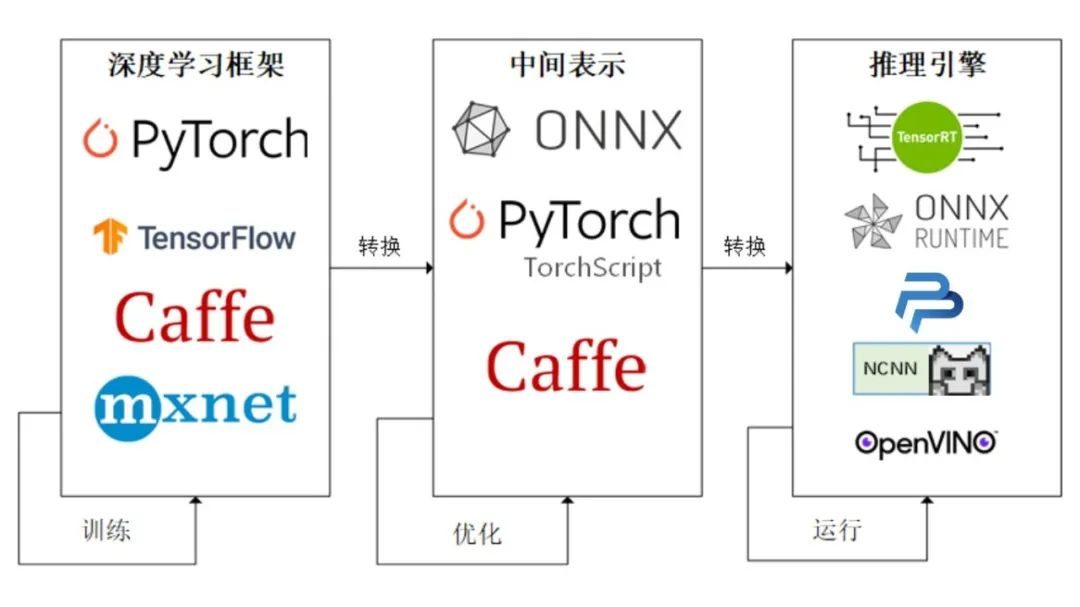
\includegraphics[width=0.7\linewidth]{imgs/pipeline.jpg}
    \caption{模型转换与推理流程}
    \label{fig:pipeline}
\end{figure}

如图 \ref{fig:pipeline} 所示,实验采用以下步骤:
\begin{enumerate}
    \item 将所有模型统一转换为 ONNX 格式
    \item 使用 ONNX Runtime 作为统一的推理引擎
    \item 在 CPU 上进行模型推理
\end{enumerate}

\subsubsection{评估指标}
为了全面评估各模型在端侧部署场景下的实际表现,本实验设计了一套多维度的评估体系,从模型性能、资源消耗和实时性三个关键维度进行量化分析:

\begin{itemize}
    \item \textbf{检测精度}:采用标准评估方法计算模型在 WIDER FACE 验证集的平均精度(Average Precision, AP),该指标反映了模型在不同难度场景下的检测能力。同时,为了评估模型在实际应用场景中的表现,我们在自建的 light\_face 数据集上计算平均精度均值(mean Average Precision, mAP),该指标能更好地反映模型在端侧实际应用场景下的检测效果

    \item \textbf{计算效率}:基于 ONNX Runtime 推理引擎,在统一的硬件环境下测试模型的每秒处理帧数(Frames Per Second, FPS)。该指标直接反映了模型的实时处理能力,对于需要实时响应的端侧应用具有重要参考价值

    \item \textbf{模型大小}:测量模型转换为 ONNX 格式后的文件大小。考虑到端侧设备存储空间和内存资源的限制,模型大小是一个重要的部署约束指标。此外,模型大小通常与其参数量和计算复杂度呈正相关,因此也间接反映了模型的计算资源需求
\end{itemize}

这套评估体系不仅考虑了模型的检测性能,还充分考虑了端侧部署的实际约束,能够为不同应用场景下的模型选择提供全面的参考依据。
\subsection{实验数据集}
本实验采用了两个互补性的数据集进行全面评估:WIDER FACE 验证集作为标准基准数据集,以及专门构建的 light\_face 数据集用于模拟实际应用场景。这种双数据集评估方案既保证了与学术界研究的可比性,又能验证模型在实际部署环境中的表现。

\subsubsection{WIDER FACE 验证集}
WIDER FACE\cite{yang2016wider} 是人脸检测领域最具权威性的标准基准数据集之一,具有以下显著特征:
\begin{itemize}
    \item \textbf{数据规模}:包含 32,203 张图像和 393,703 个人脸标注,是当前最大规模的人脸检测数据集之一
    \item \textbf{场景多样性}:涵盖了 61 个不同的事件类别,包括室内外、日间夜晚等各种真实场景
    \item \textbf{挑战性}:图像中的人脸呈现出尺度、姿态、表情、遮挡、光照等多维度的变化
    \item \textbf{难度分级}:基于人脸检测难度将数据划分为简单(Easy)、中等(Medium)和困难(Hard)三个子集,其中:
    \begin{itemize}
        \item Easy:包含大尺寸且清晰可见的人脸
        \item Medium:包含中等尺寸且部分遮挡的人脸
        \item Hard:包含小尺寸、严重遮挡或模糊的人脸
    \end{itemize}
    \item \textbf{评估标准化}:提供统一的评估工具和标准化的评估流程,确保不同研究之间结果的可比性
    \item \textbf{学术影响力}:被广泛应用于学术研究和算法竞赛,是评估人脸检测算法性能的金标准
\end{itemize}

\subsubsection{自建单人人脸数据集 light\_face}
为了更准确地评估模型在端侧实际应用场景中的性能表现,我们设计并构建了专门的单人人脸数据集 light\_face:
\begin{itemize}
    \item \textbf{数据采集}:
    \begin{itemize}
        \item 使用主流端侧设备(笔记本电脑和智能手机)的前置摄像头进行视频采集
        \item 采集环境包括办公室、家庭等典型室内场景
        \item 采集时间覆盖白天和夜晚,确保光照条件的多样性
    \end{itemize}
    \item \textbf{数据特征}:
    \begin{itemize}
        \item 图像分辨率:与主流端侧设备前置摄像头分辨率一致(1280×720)
        \item 人脸姿态:覆盖±45°的水平和垂直转角范围
        \item 光照条件:包括自然光、室内灯光、逆光等多种情况
    \end{itemize}
    \item \textbf{数据处理}:
    \begin{itemize}
        \item 从原始视频中以 2fps 的采样率提取关键帧
        \item 最终构建包含 700+ 张图像的数据集
        \item 使用腾讯云人脸检测 API 进行标注
    \end{itemize}
    \item \textbf{应用价值}:该数据集特征与实际端侧应用场景高度吻合,适用于评估模型在视频会议、人脸解锁、人机交互等实际应用中的性能表现。同时,使用腾讯云人脸检测 API 作为标注工具,可以将其检测结果作为工业级模型的基准,用于评估轻量级模型与工业级模型之间的性能差距
\end{itemize}

\subsection{实验结果与分析}
\subsubsection{推理效果展示}

\begin{figure}[htbp]
    \centering
    \begin{subfigure}[b]{0.48\textwidth}
        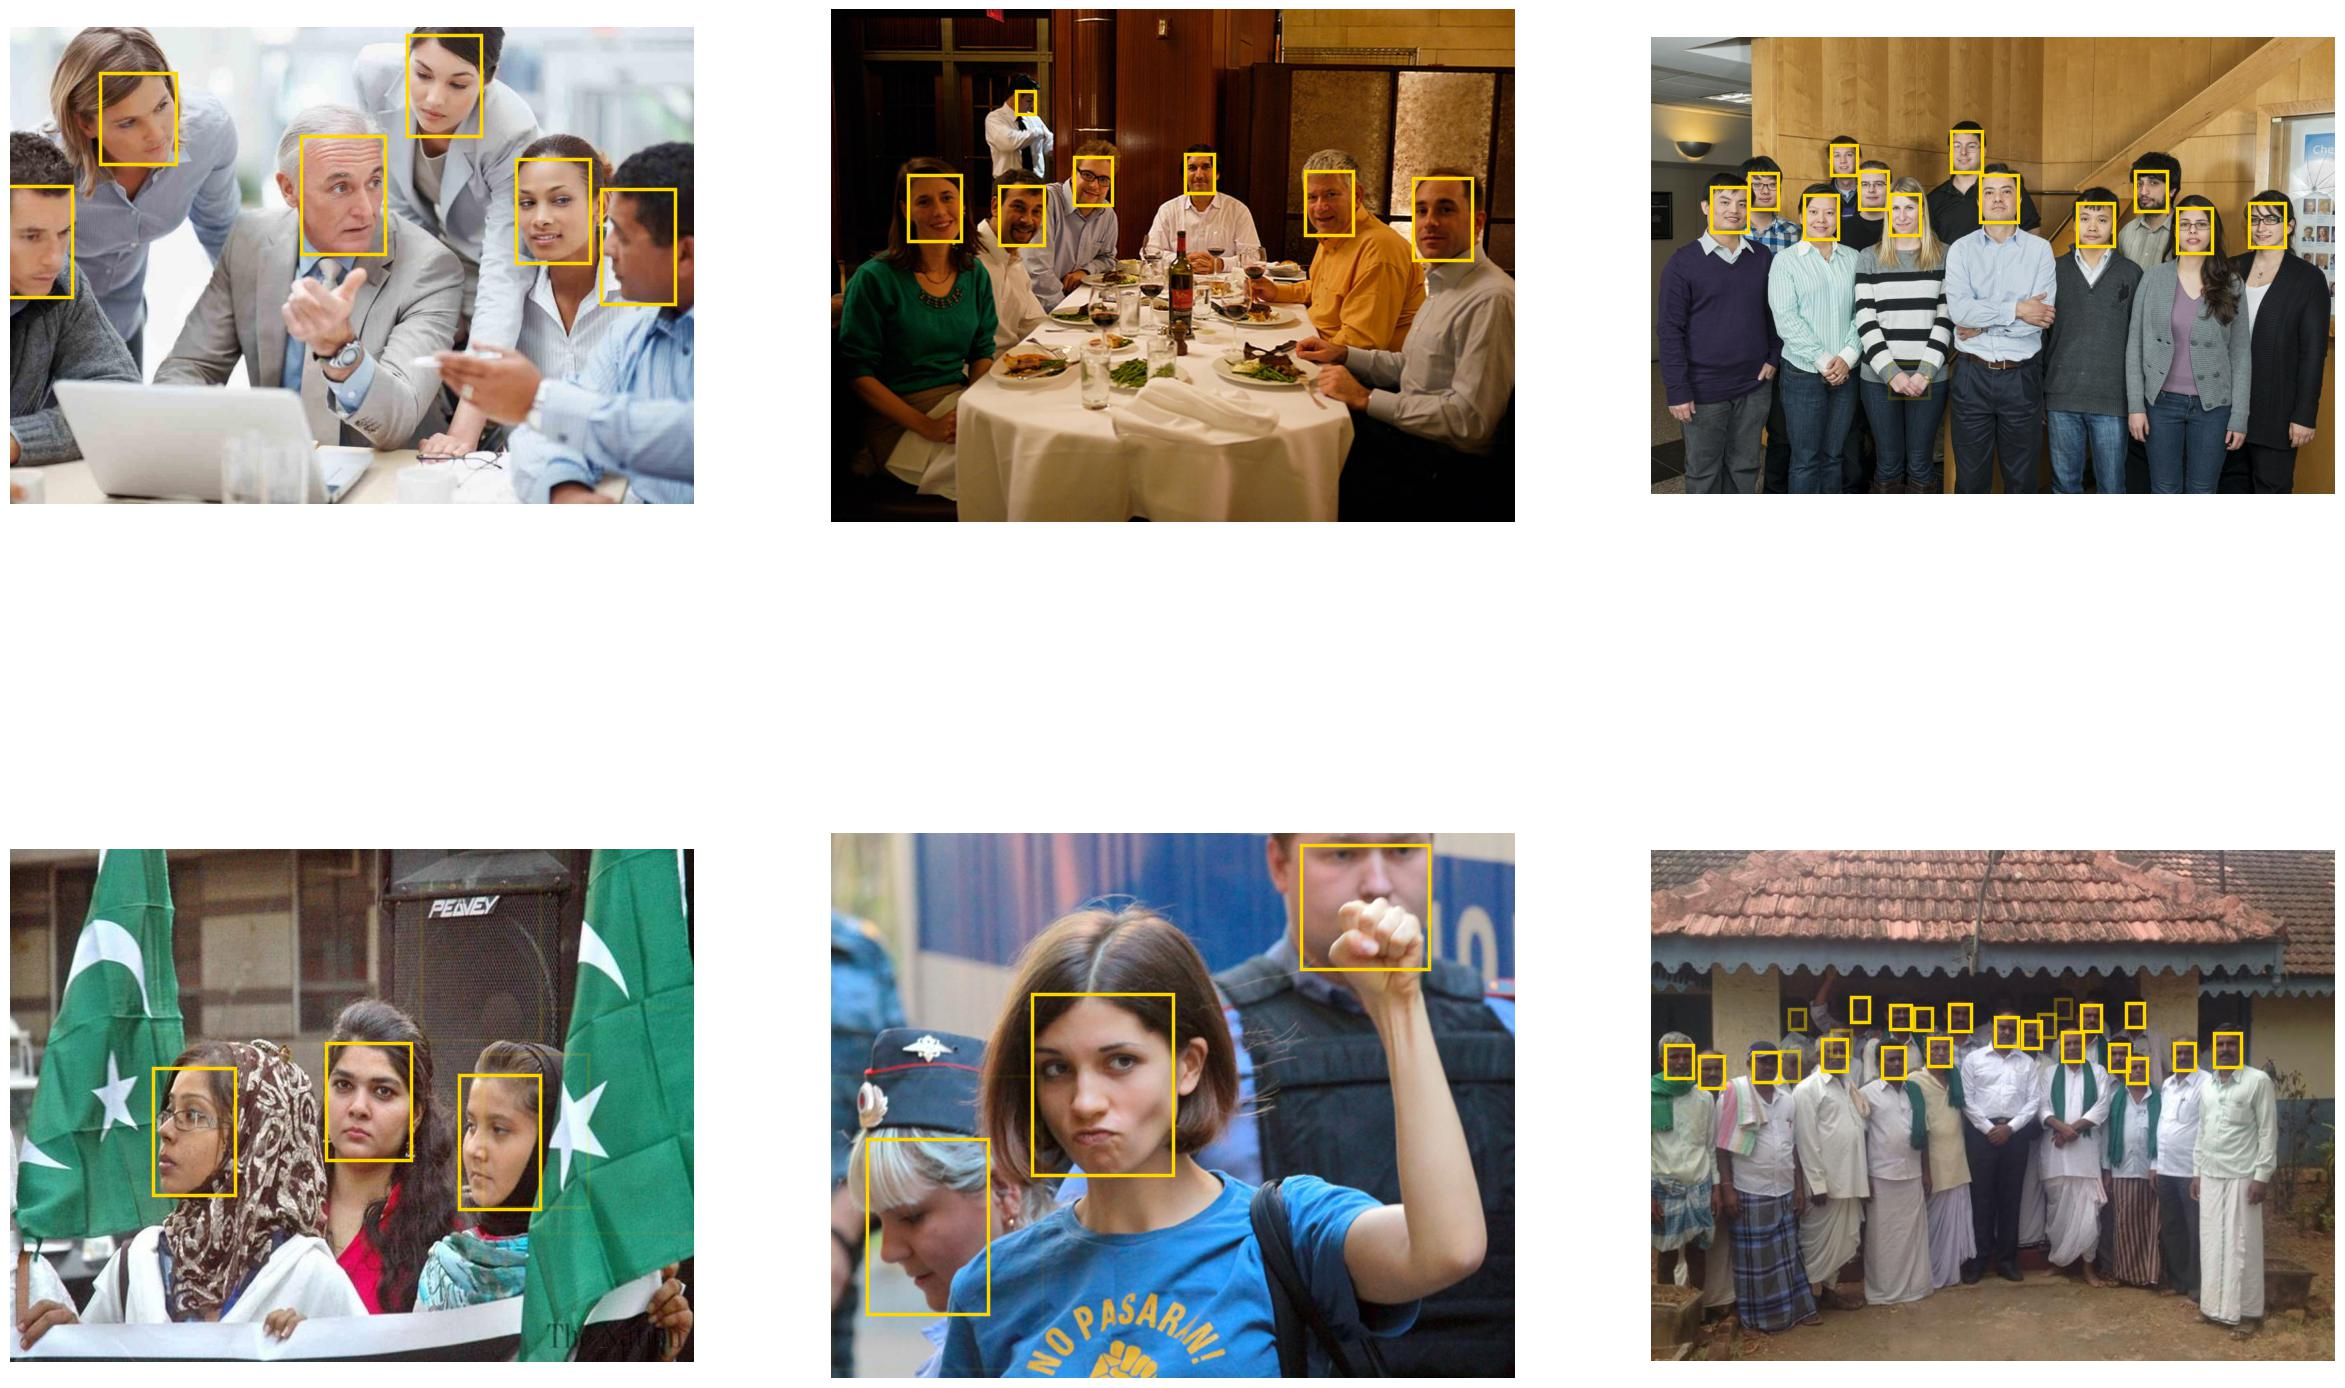
\includegraphics[width=\textwidth]{imgs/infer_result/retinaface_mv1_0.25.jpg}
        \caption{RetinaFace-MobileNet0.25}
    \end{subfigure}
    \hfill
    \begin{subfigure}[b]{0.48\textwidth}
        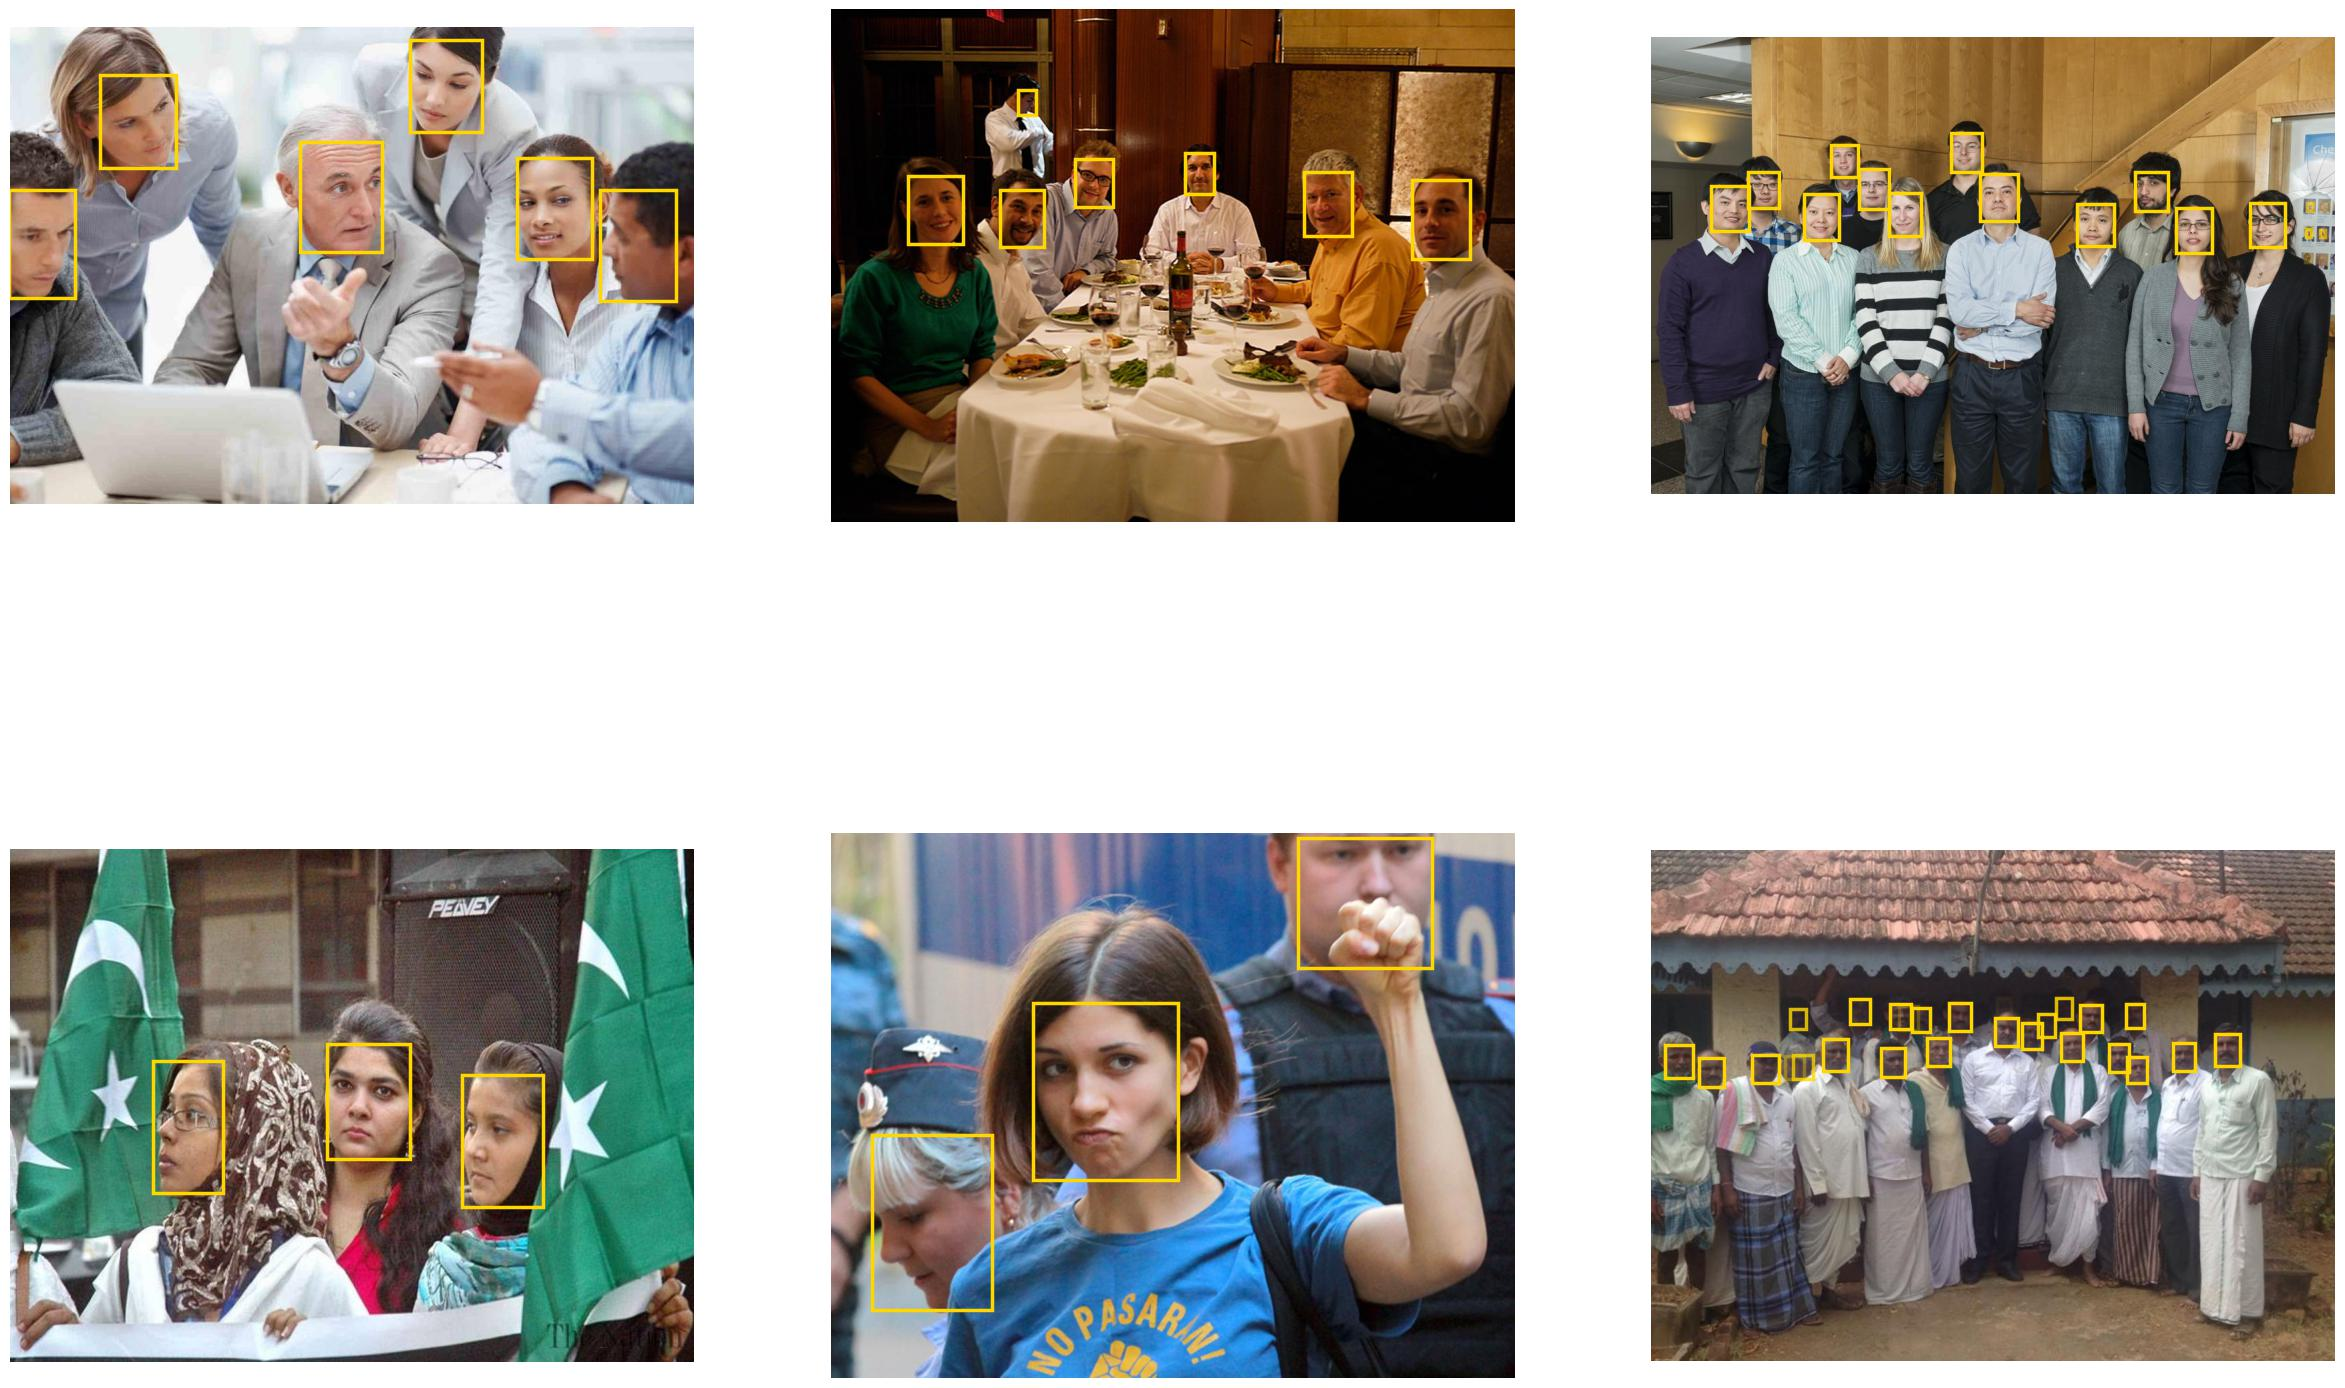
\includegraphics[width=\textwidth]{imgs/infer_result/retinaface_mv2.jpg}
        \caption{RetinaFace-MobileNetV2}
    \end{subfigure}
    \caption{RetinaFace 系列模型推理效果}
    \label{fig:infer_retinaface}
\end{figure}

\begin{figure}[htbp]
    \centering
    \begin{subfigure}[b]{0.48\textwidth}
        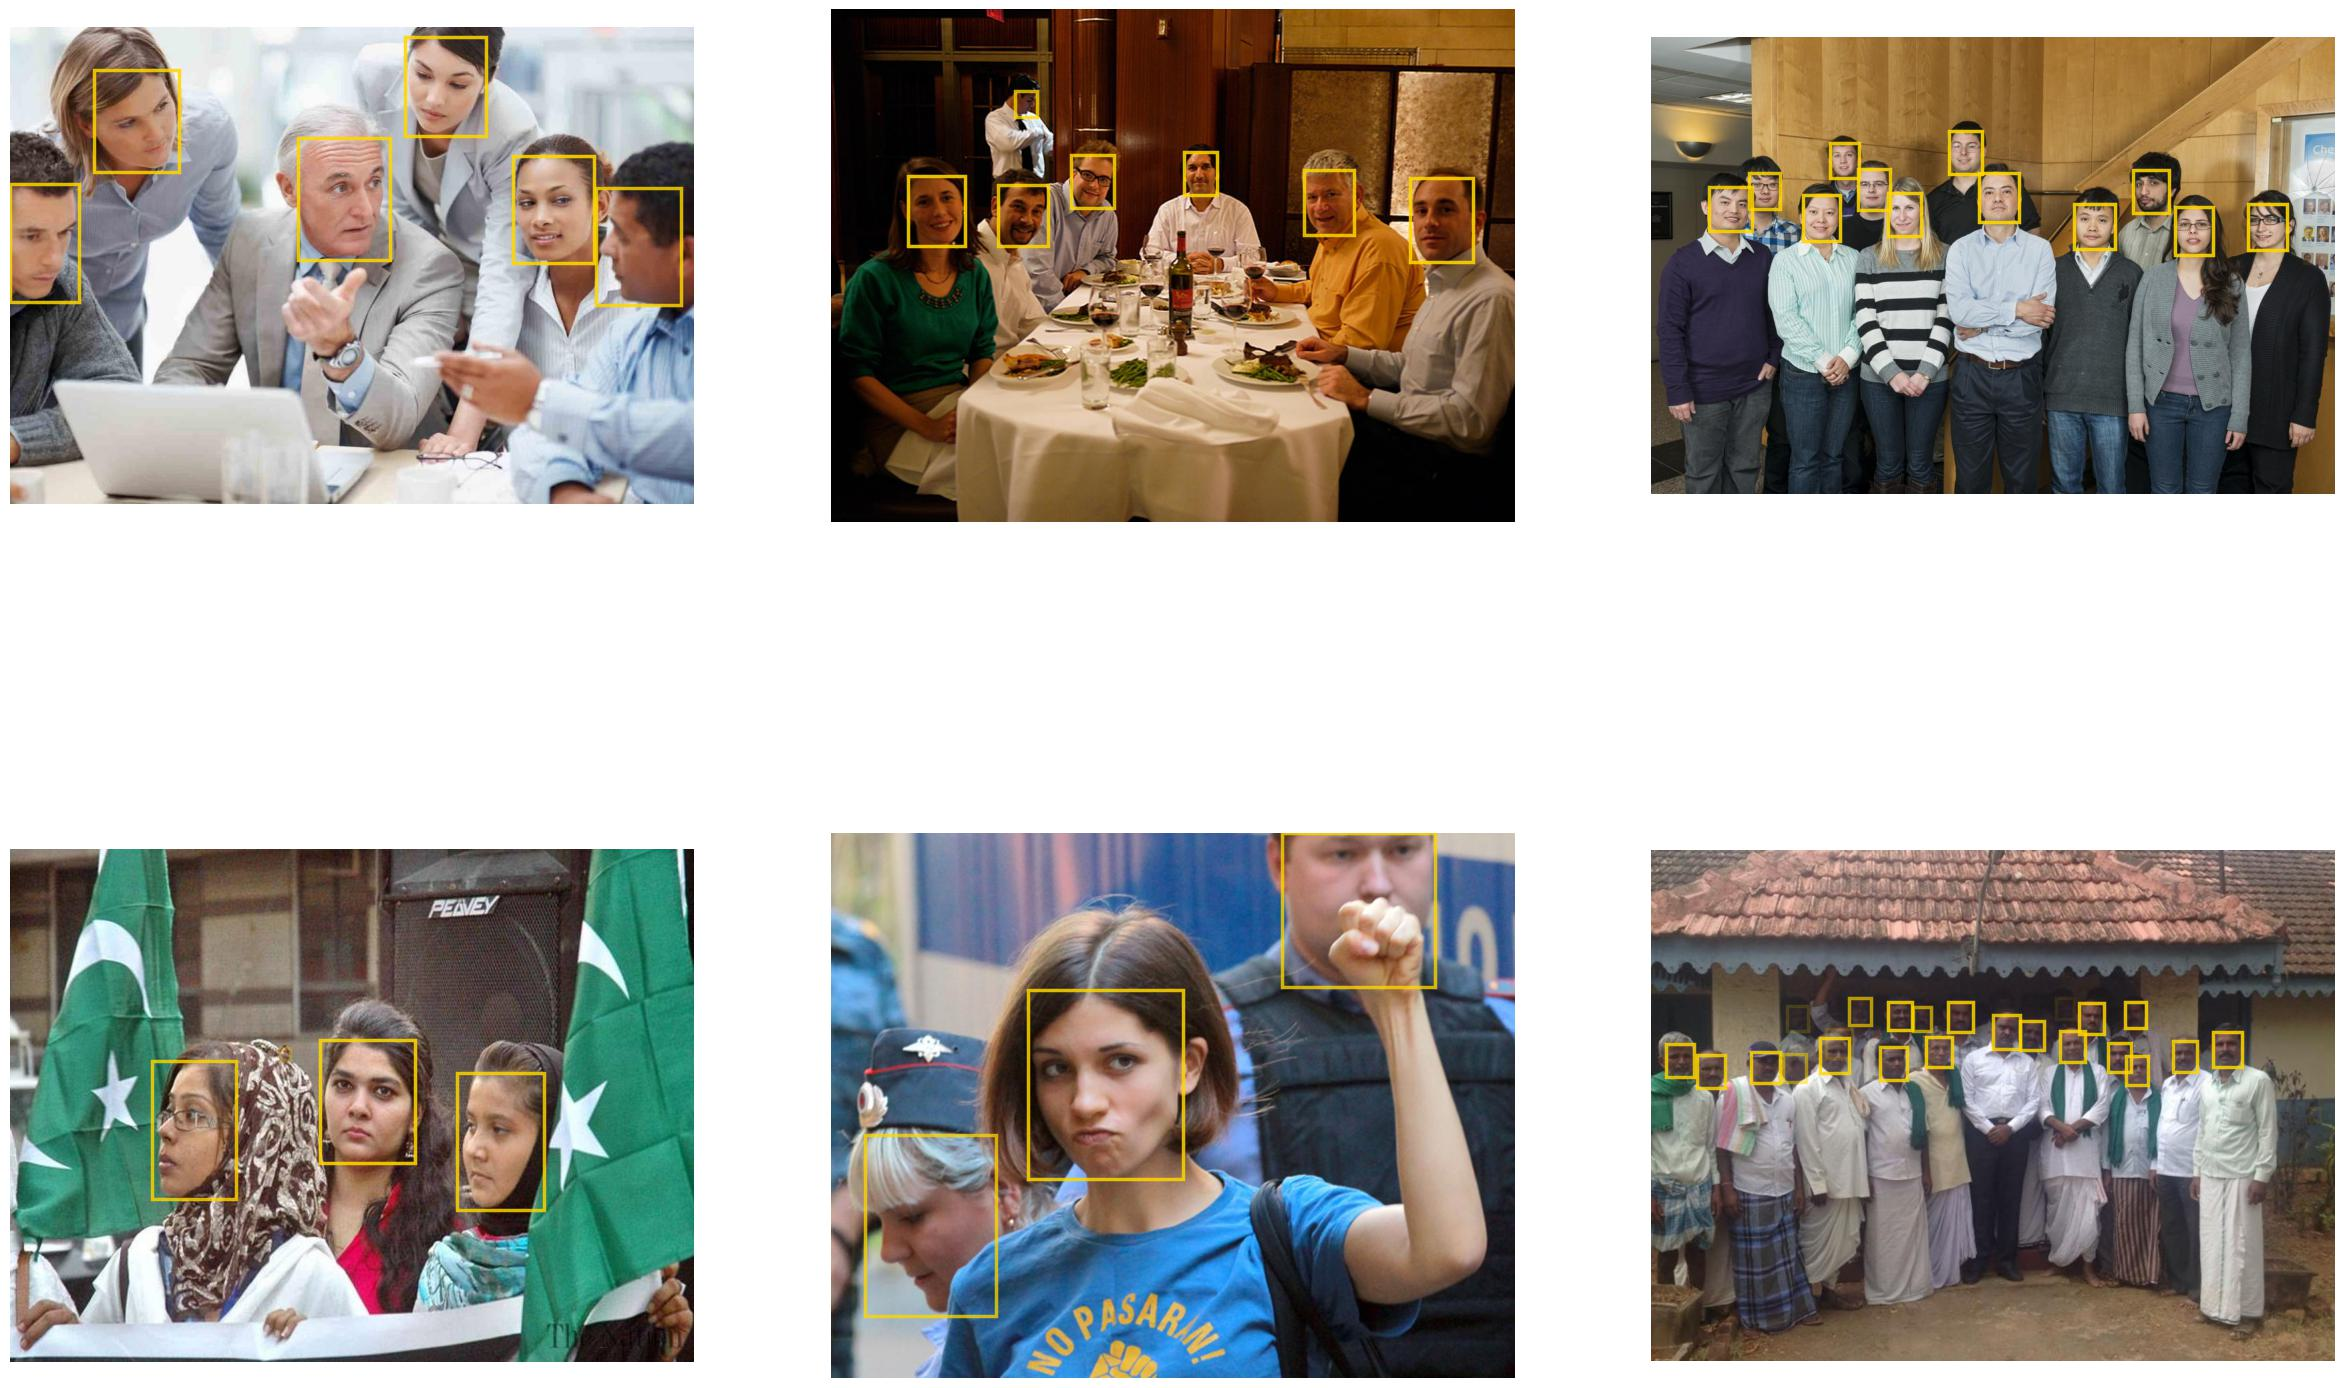
\includegraphics[width=\textwidth]{imgs/infer_result/yolov5n_0.5_face.jpg}
        \caption{YOLOv5n-0.5-Face}
    \end{subfigure}
    \hfill
    \begin{subfigure}[b]{0.48\textwidth}
        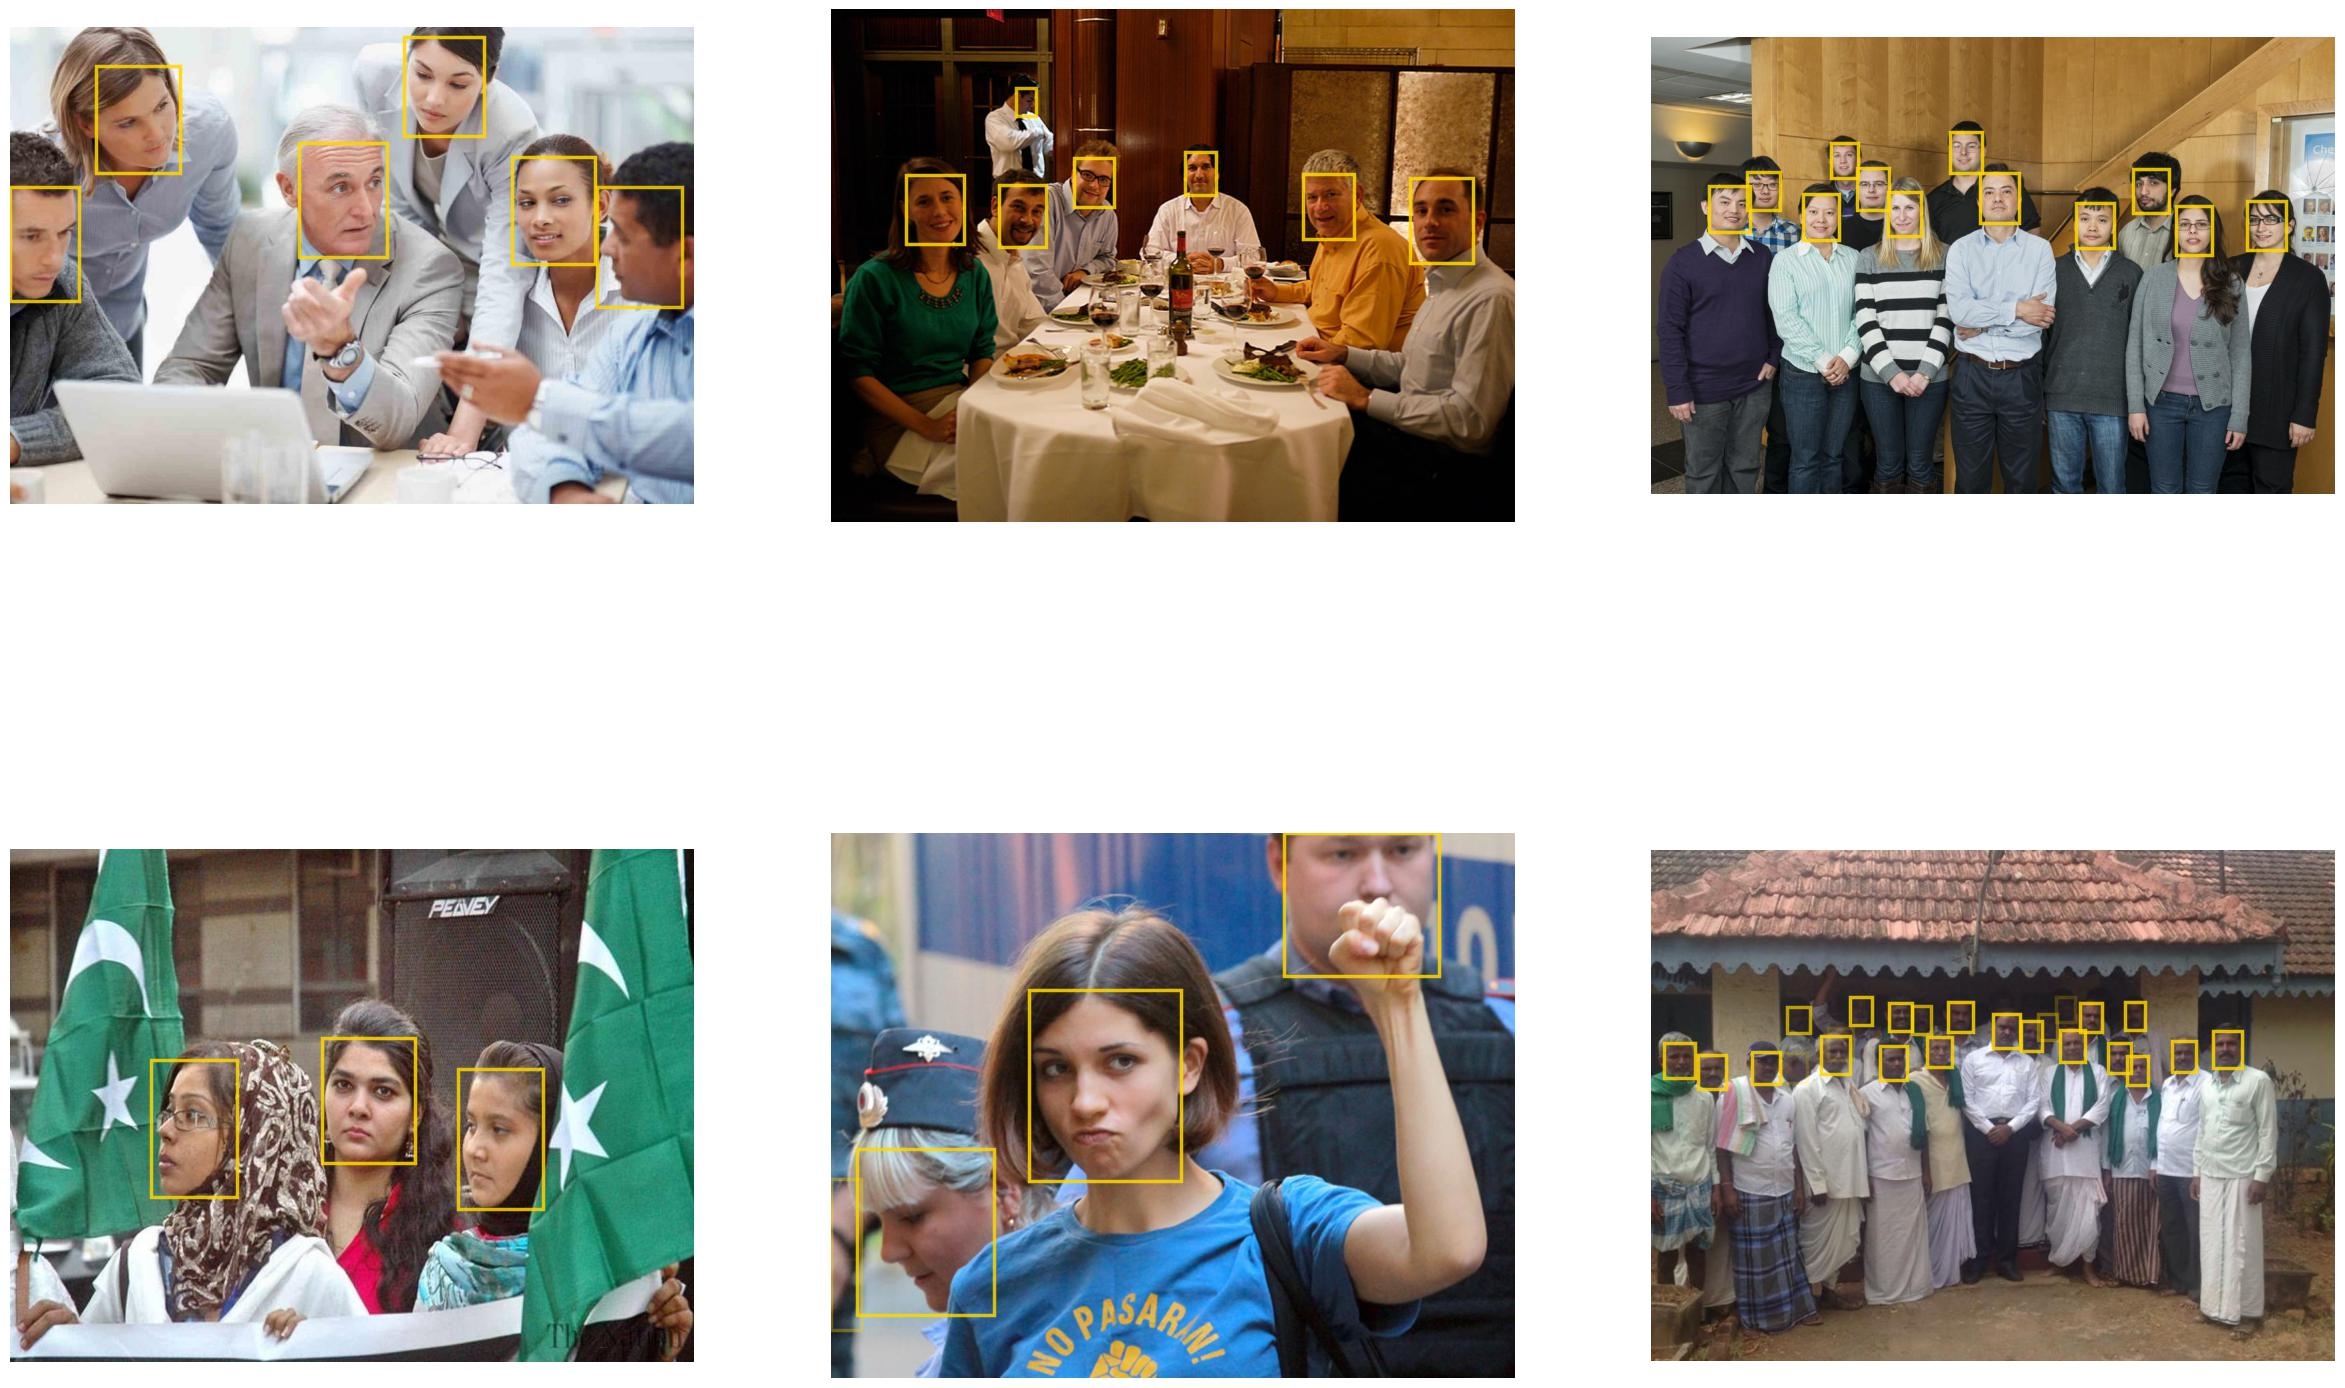
\includegraphics[width=\textwidth]{imgs/infer_result/yolov5n_face.jpg}
        \caption{YOLOv5n-Face}
    \end{subfigure}
    \caption{YOLOv5Face 系列模型推理效果}
    \label{fig:infer_yolov5face}
\end{figure}
\begin{figure}[htbp]
    \centering
    \begin{subfigure}[b]{0.32\textwidth}
        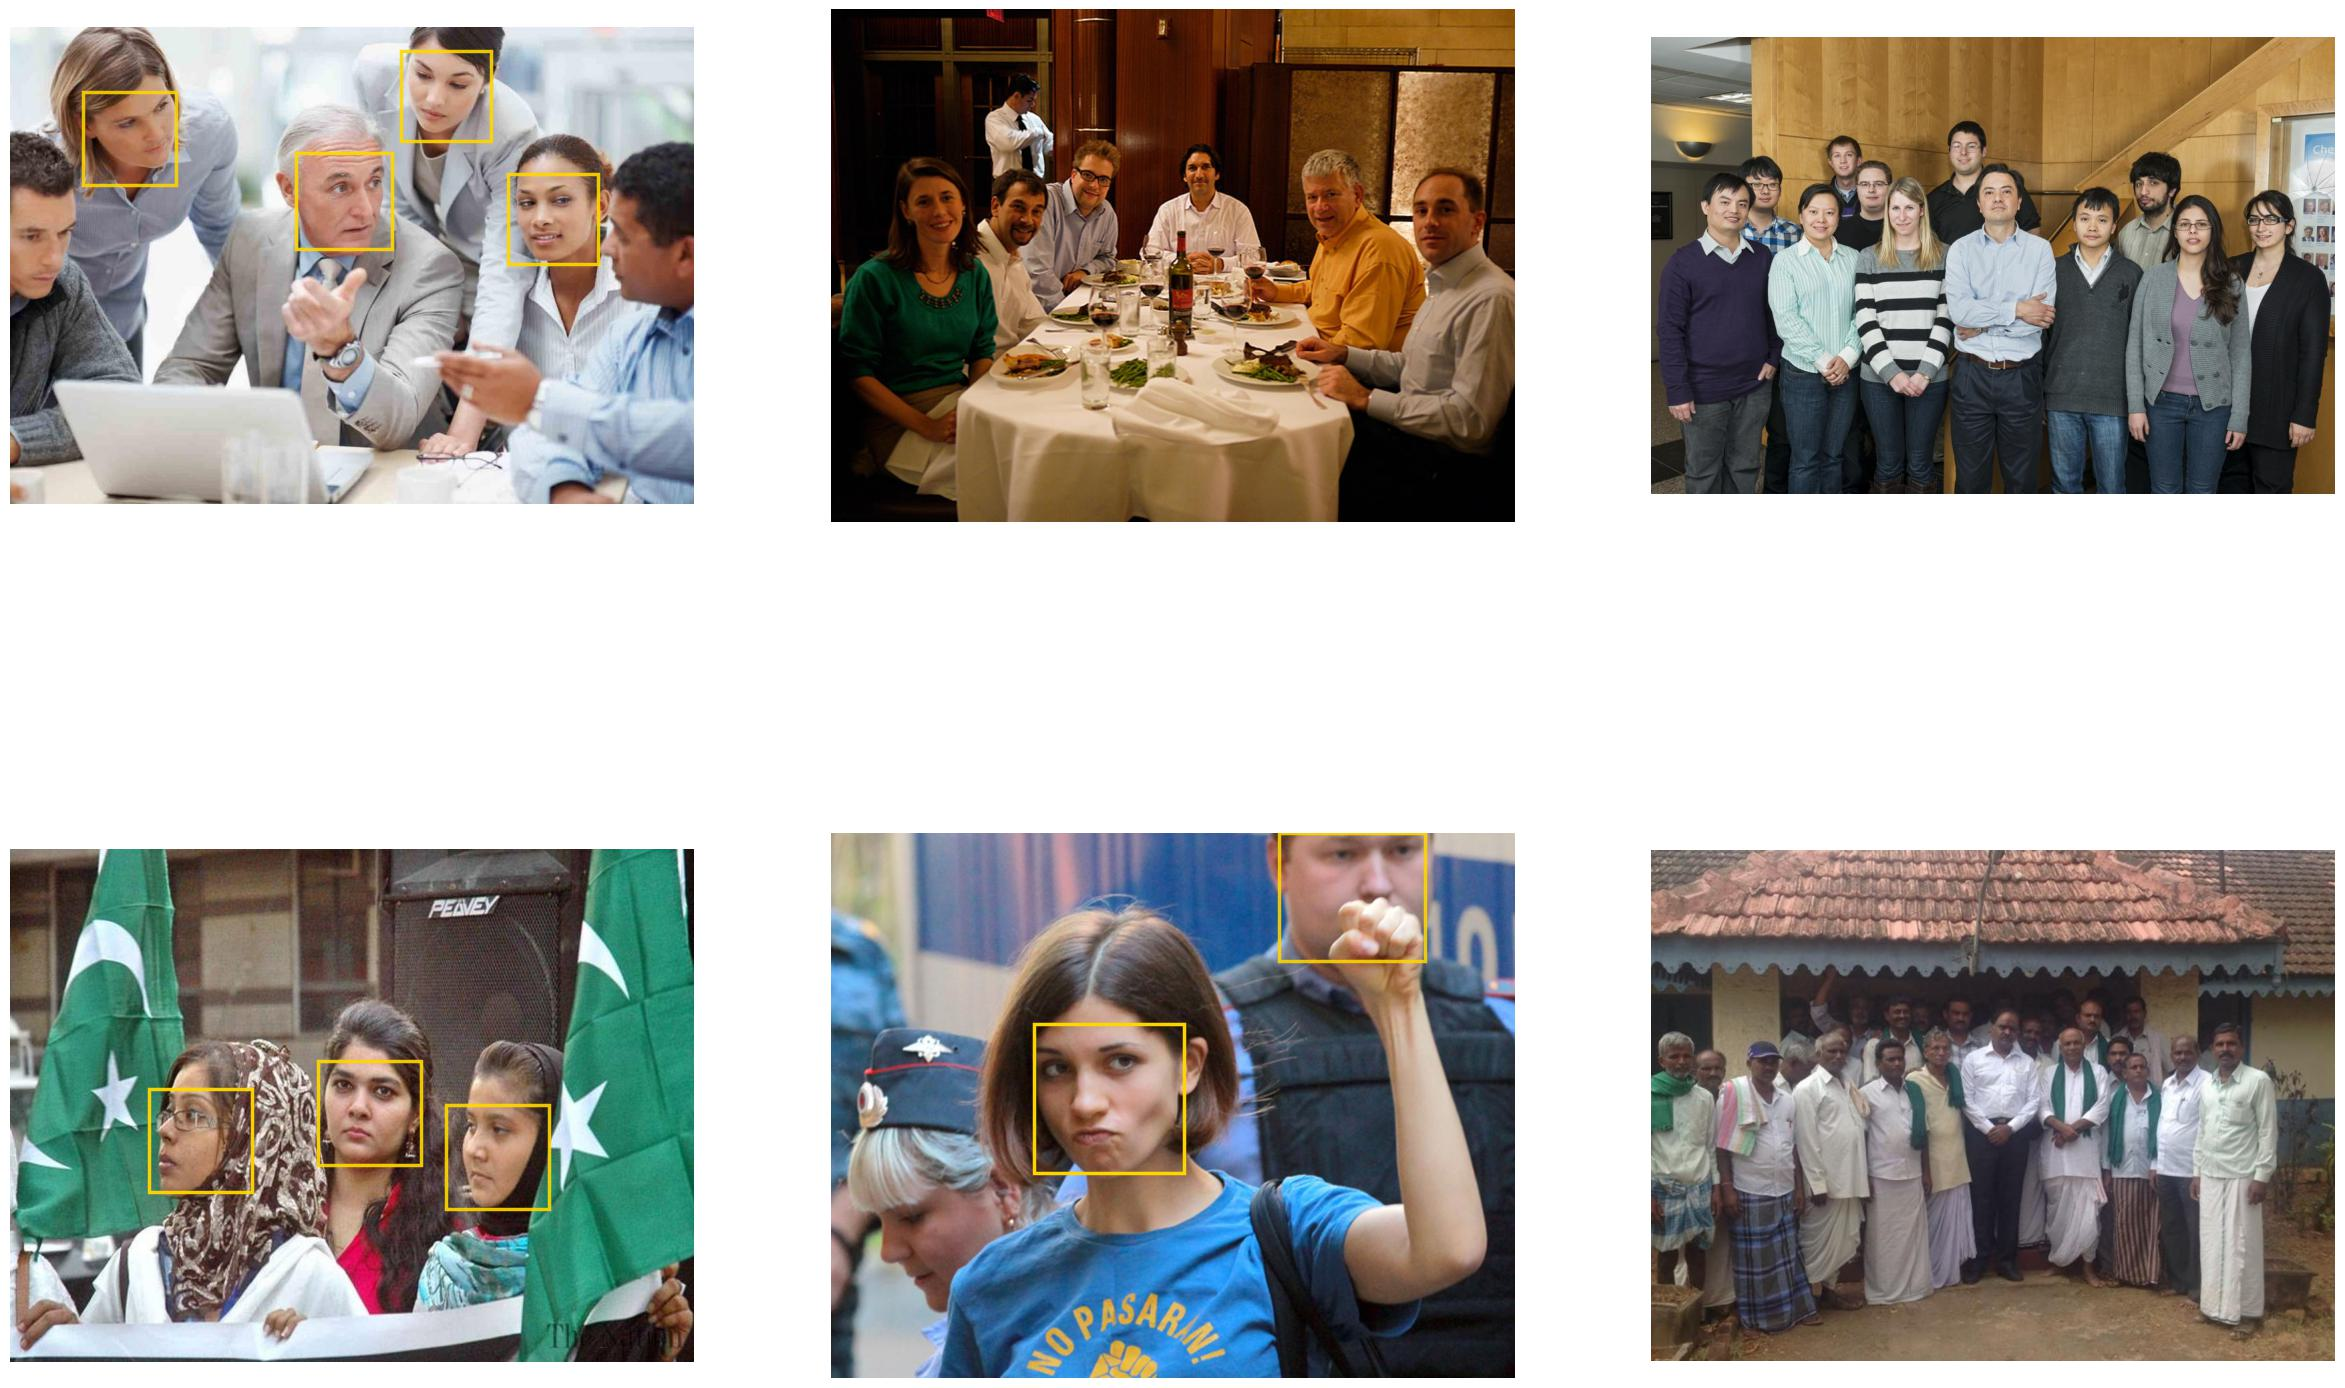
\includegraphics[width=\textwidth]{imgs/infer_result/blazeface_128.jpg}
        \caption{BlazeFace-128}
    \end{subfigure}
    \hfill
    \begin{subfigure}[b]{0.32\textwidth}
        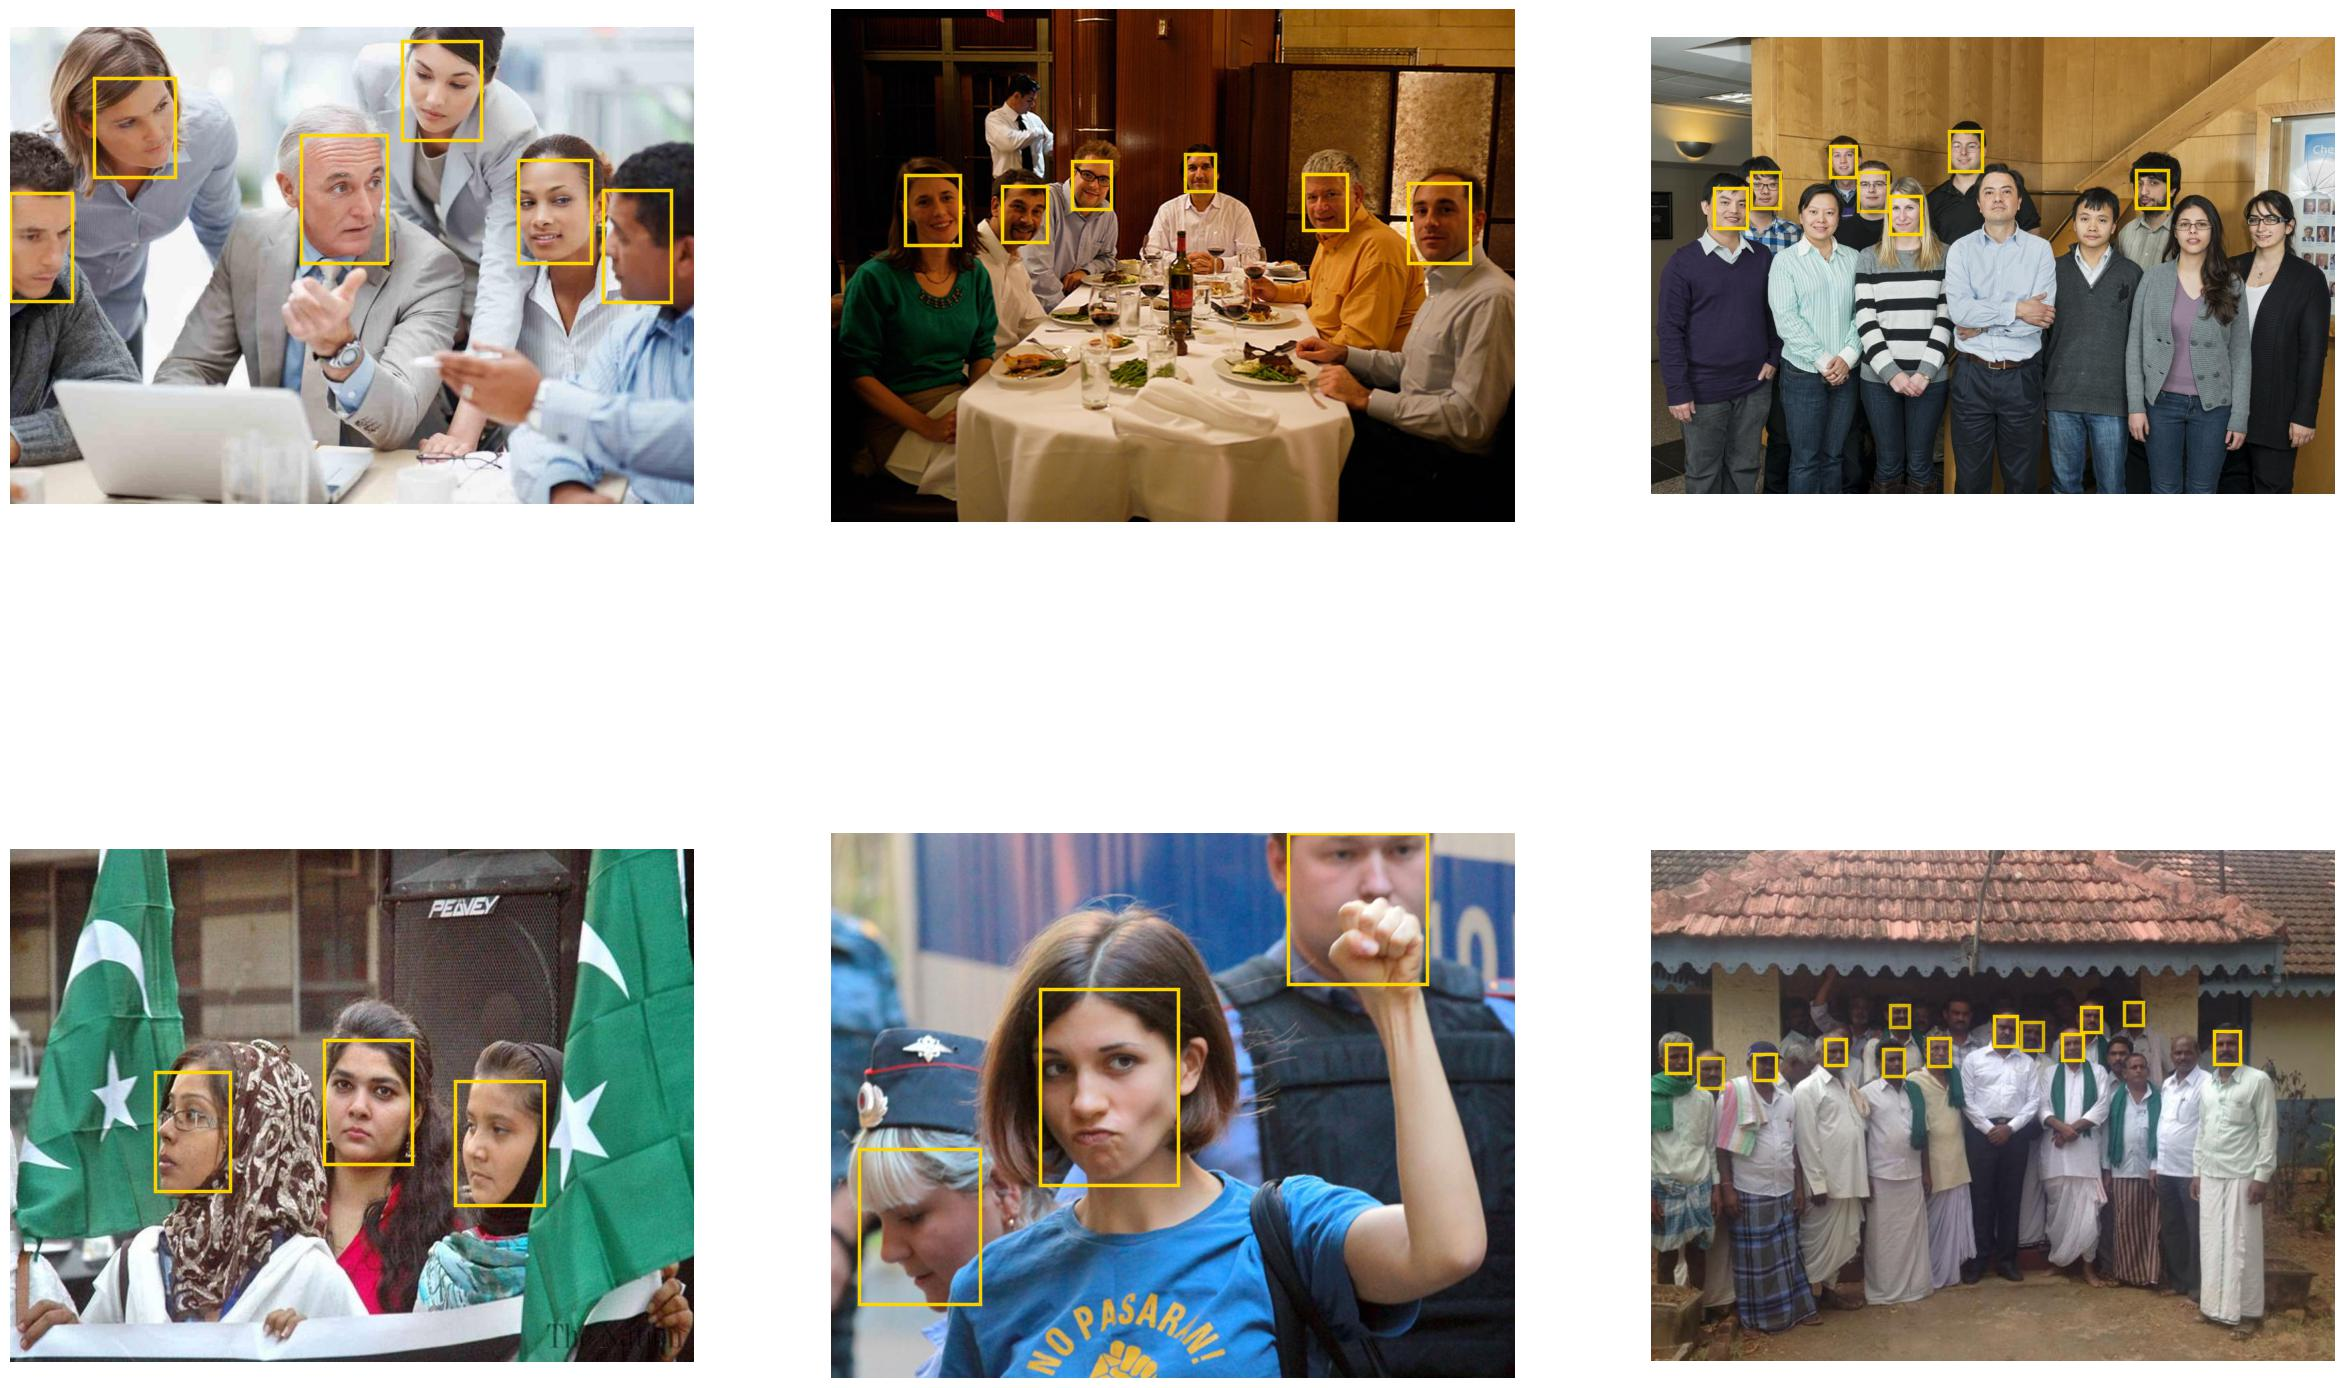
\includegraphics[width=\textwidth]{imgs/infer_result/blazeface_320.jpg}
        \caption{BlazeFace-320}
    \end{subfigure}
    \hfill
    \begin{subfigure}[b]{0.32\textwidth}
        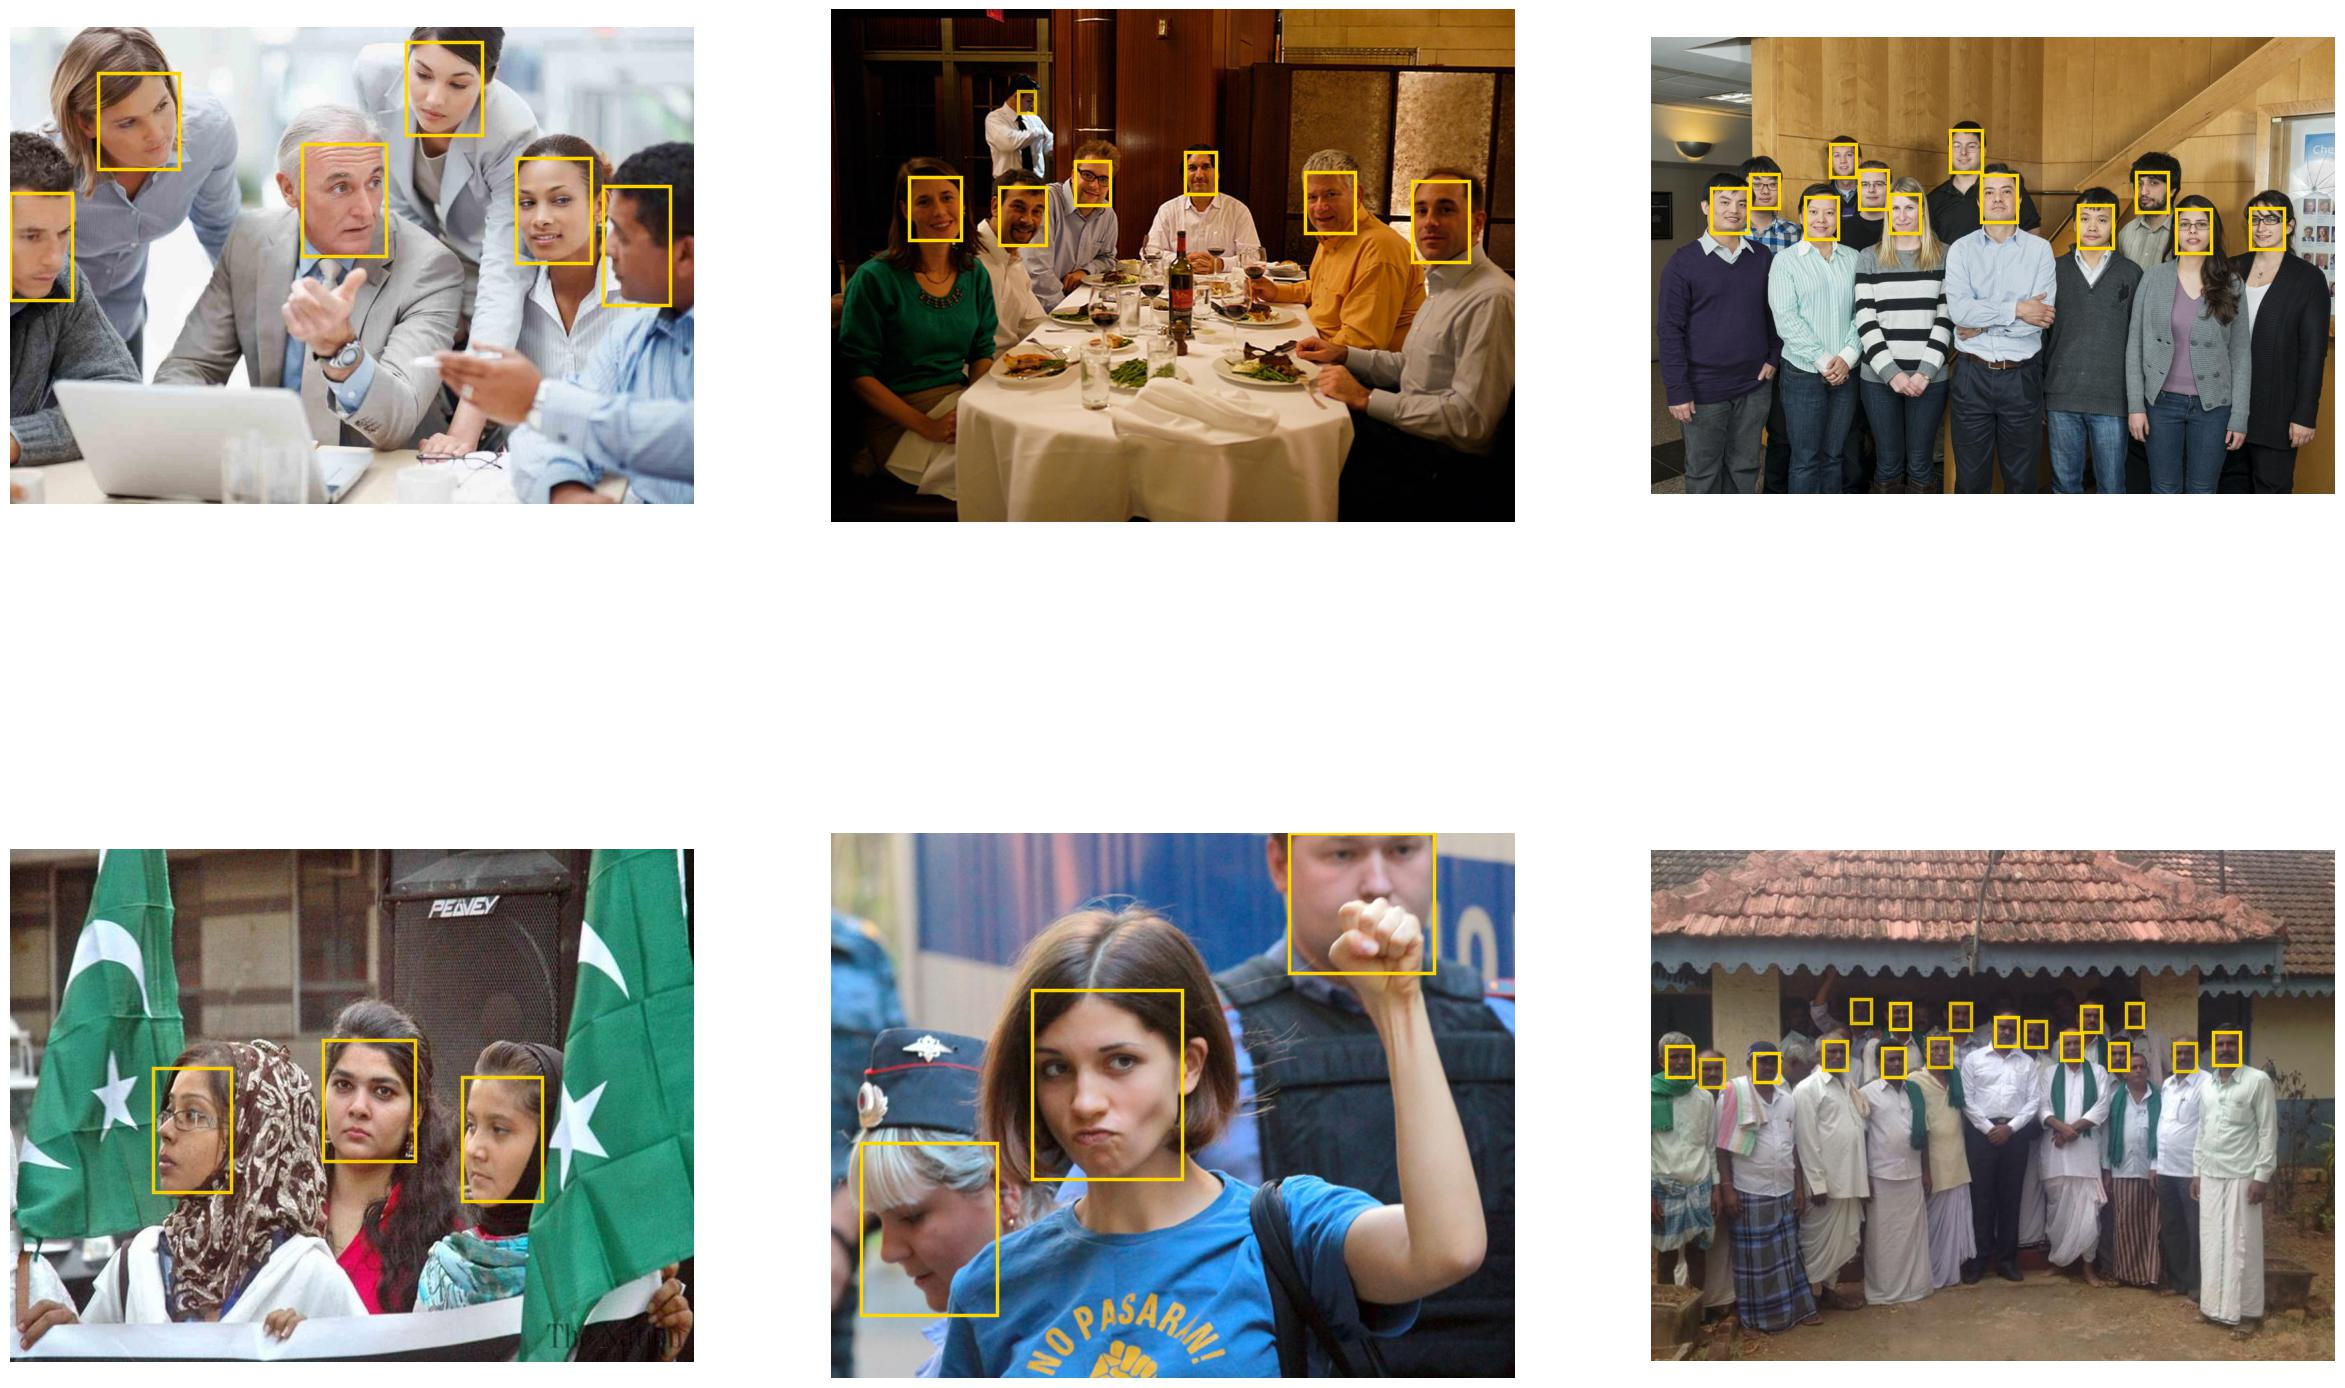
\includegraphics[width=\textwidth]{imgs/infer_result/blazeface_640.jpg}
        \caption{BlazeFace-640}
    \end{subfigure}
    \caption{BlazeFace 系列模型推理效果}
    \label{fig:infer_blazeface}
\end{figure}

\subsubsection{性能指标对比}

\begin{table}[!ht]
    \centering
    \begin{tabular}{l|c|c|c|c|c|c}
        \hline
        Model & Size(MB) & FPS & Easy & Medium & Hard & light\_face \\
        \hline
        retinaface\_mv1 & 1.66 & 8.68 & 0.91 & 0.88 & 0.73 & \underline{\textbf{0.991}} \\
        retinaface\_mv2 & 11.93 & 4.15 & 0.94 & \underline{\textbf{0.92}} & \underline{\textbf{0.82}} & 0.991 \\
        yolov5n\_0.5\_face & 5.65 & 22.23 & 0.91 & 0.88 & 0.75 & 0.987 \\
        yolov5n\_face & 10.51 & 12.90 & \underline{\textbf{0.94}} & 0.92 & 0.81 & 0.987 \\
        blazeface\_128 & \underline{\textbf{0.44}} & \underline{\textbf{70.79}} & 0.18 & 0.10 & 0.04 & 0.667 \\
        blazeface\_320 & 0.68 & 46.46 & 0.60 & 0.46 & 0.20 & 0.932 \\
        blazeface\_640 & 0.68 & 16.26 & 0.80 & 0.64 & 0.35 & 0.984 \\
        \hline
    \end{tabular}
    \caption{各模型性能指标对比}
    \label{tab:model_performance}
\end{table}

表 \ref{tab:model_performance} 展示了各模型在不同评估指标上的表现,从表中数据可以观察到以下几个关键特点:
\begin{itemize}
    \item RetinaFace 和 YOLO5Face 系列在检测精度上表现优异,但模型体积较大
    \item BlazeFace 系列在速度和模型大小上具有明显优势,但精度有所牺牲
    \item YOLOv5n-0.5-face 在各项指标上表现较为均衡
\end{itemize}

\subsubsection{模型大小与推理速度分析}

\begin{figure}[htbp]
    \centering
    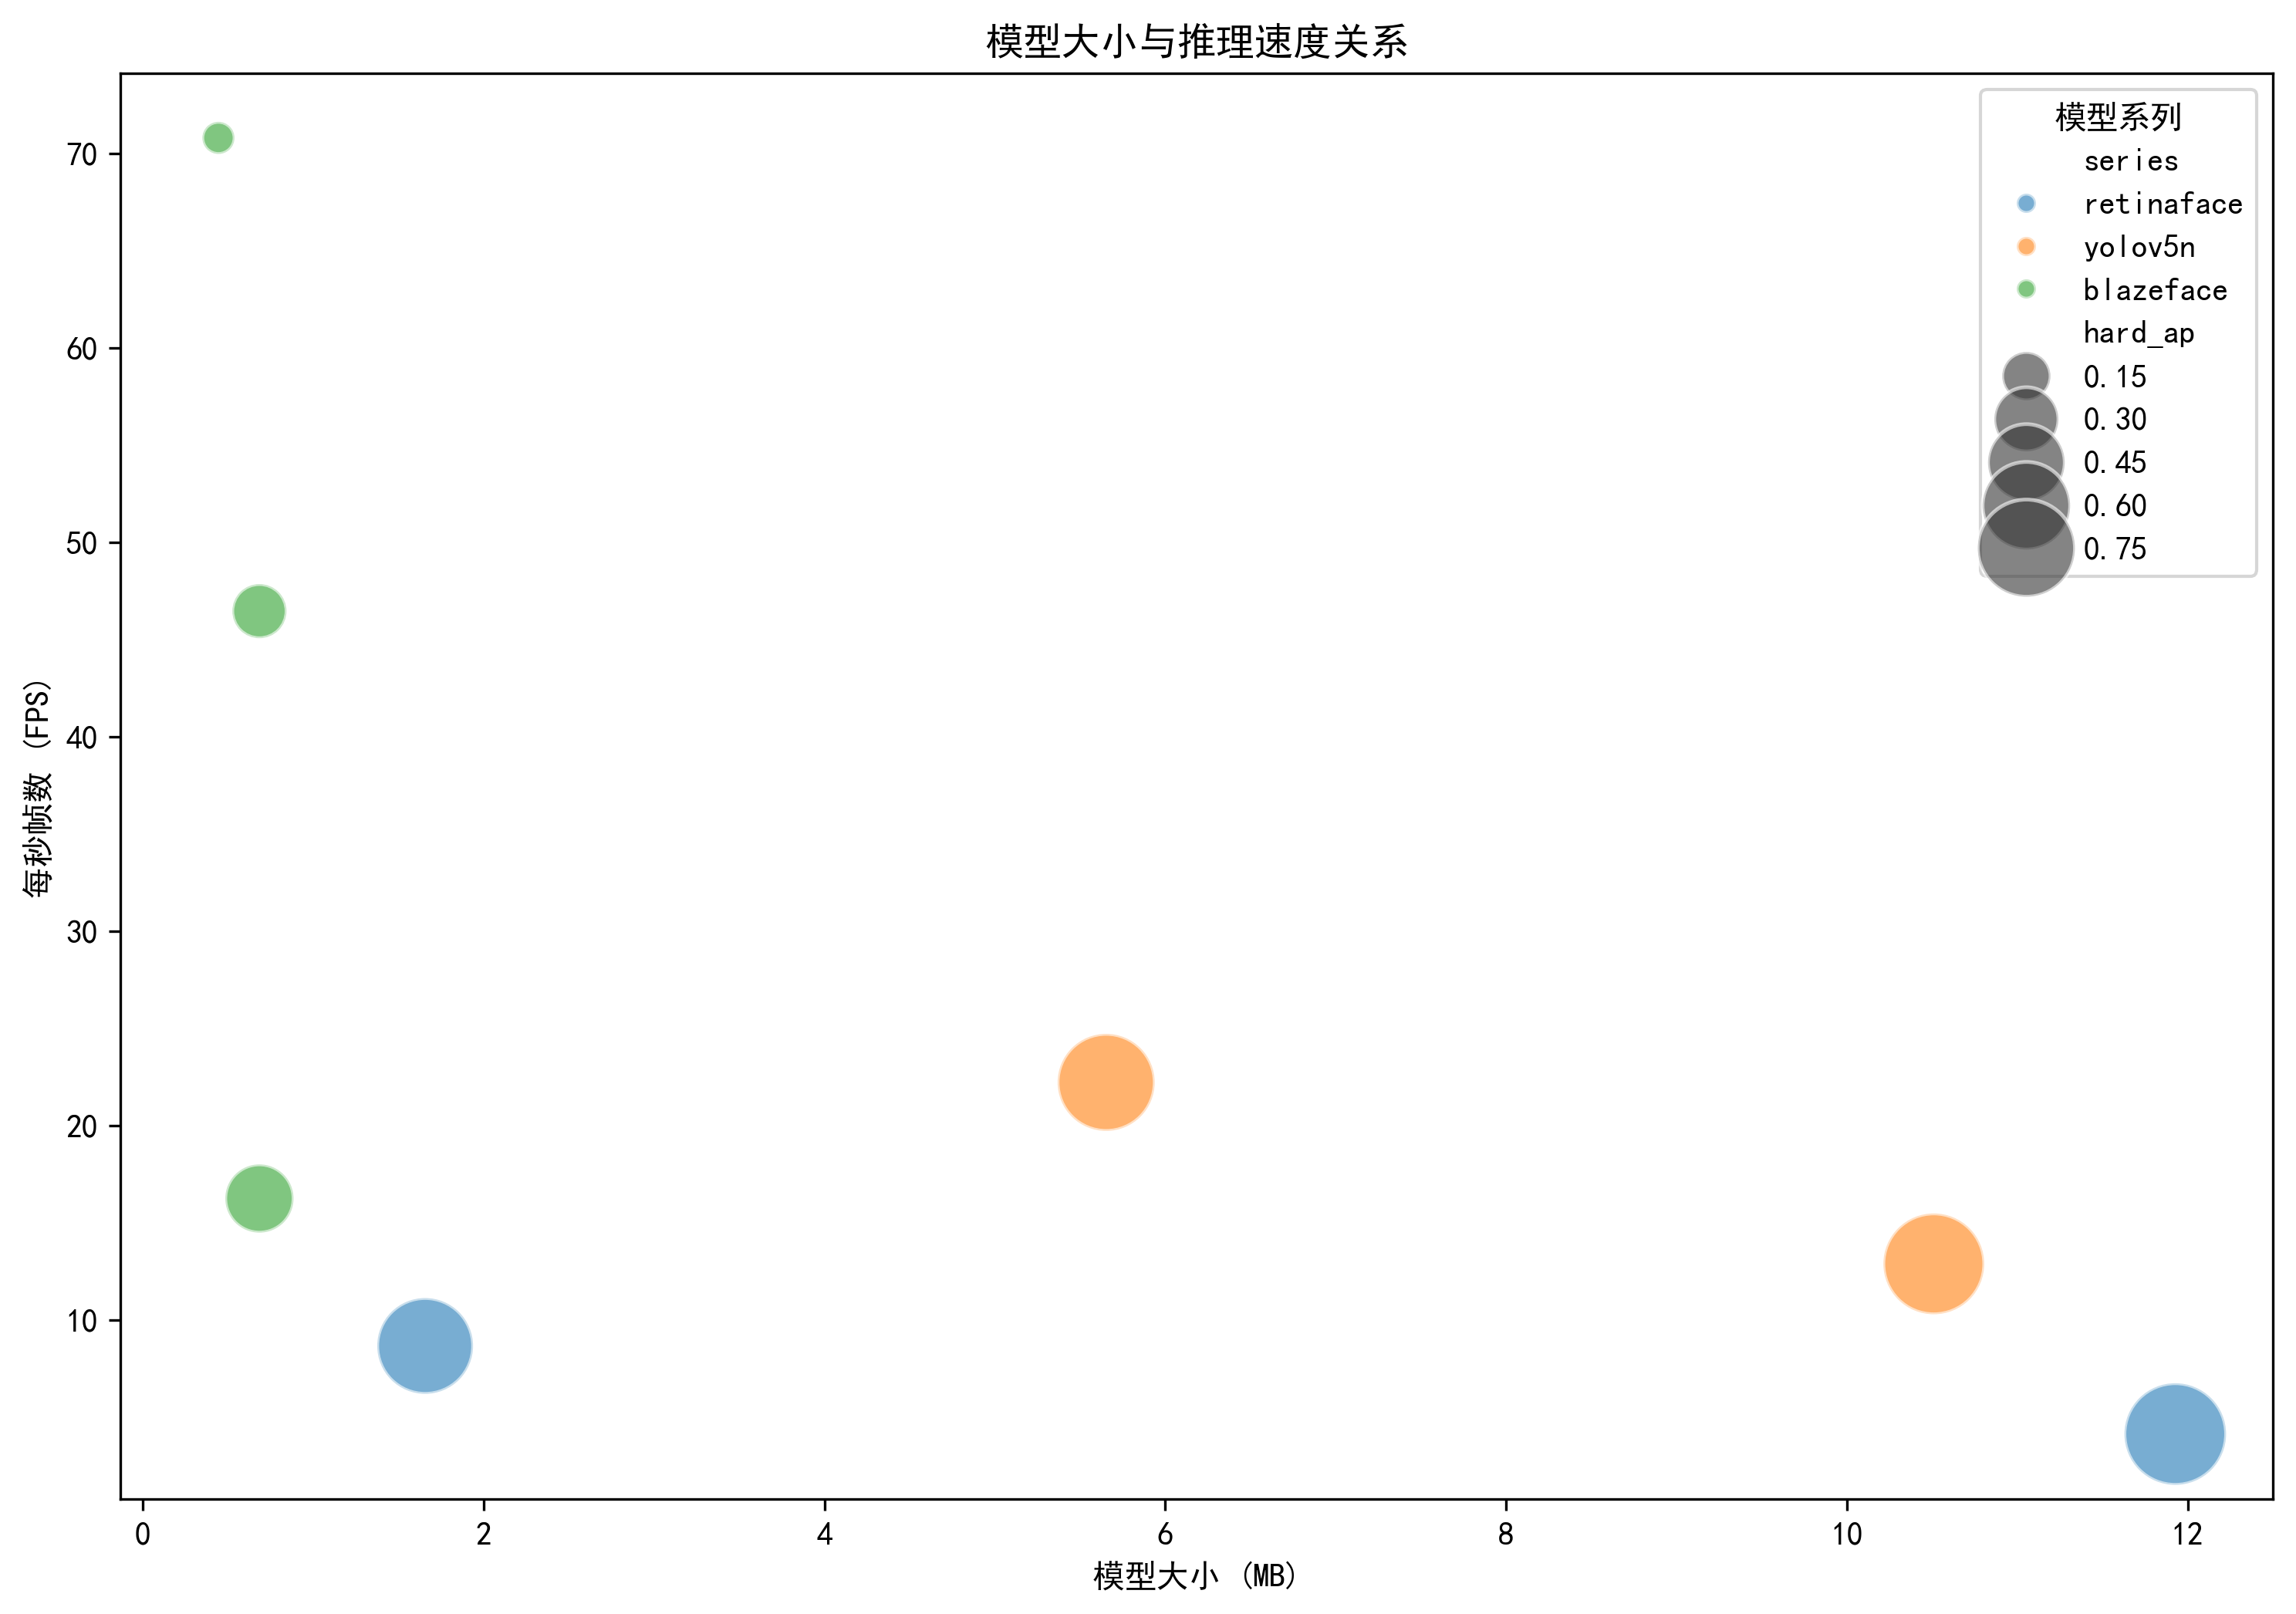
\includegraphics[width=0.8\linewidth]{imgs/size_fps.png}
    \caption{模型大小与推理速度对比}
    \label{fig:size_fps}
\end{figure}

如图 \ref{fig:size_fps} 所示,模型大小与推理速度之间存在明显的权衡关系:
\begin{itemize}
    \item BlazeFace 系列模型体积最小(<1MB),推理速度最快(最高达到 70+ FPS)
    \item RetinaFace-MobileNetV2 和 YOLOv5n-face 模型体积较大(>10MB),推理速度相对较慢
    \item YOLOv5n-0.5-face 在模型大小和推理速度上达到了较好的平衡
\end{itemize}

\subsubsection{检测精度分析}

\begin{figure}[htbp]
    \centering
    \begin{subfigure}[b]{0.48\textwidth}
        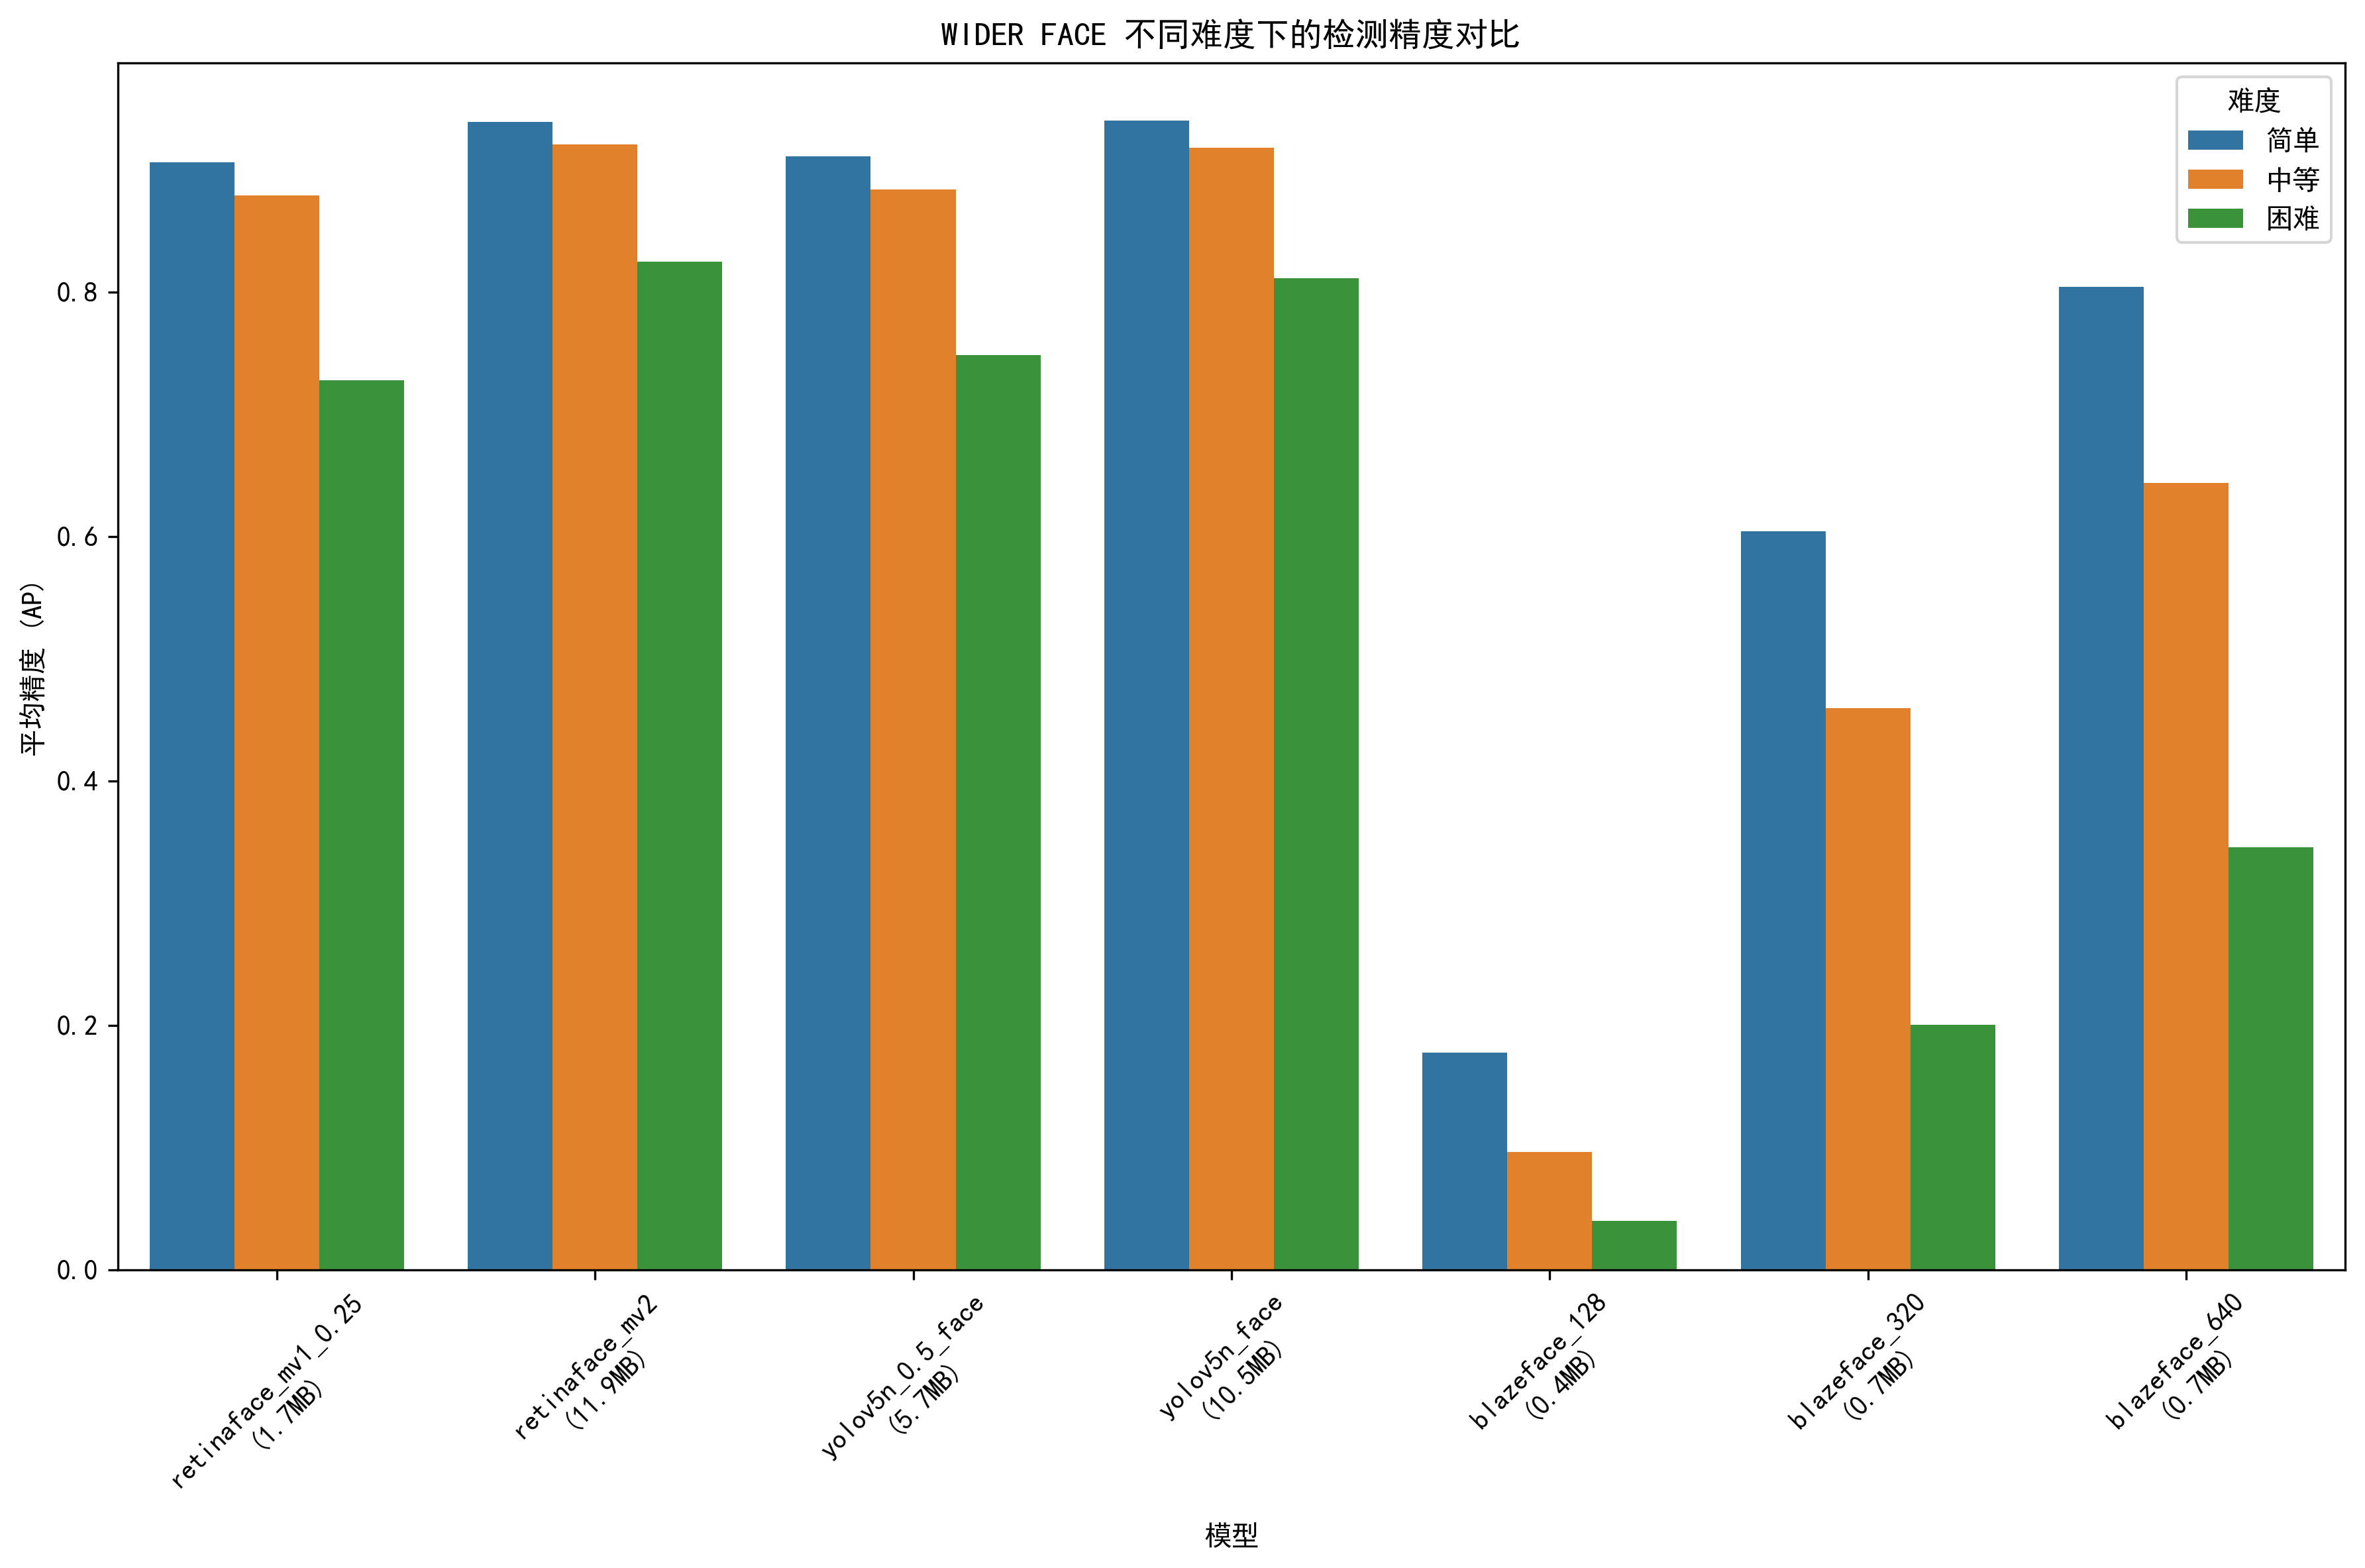
\includegraphics[width=\textwidth]{imgs/ap_comparison.png}
        \caption{不同难度级别下的检测精度}
        \label{fig:ap_comparison}
    \end{subfigure}
    \hfill
    \begin{subfigure}[b]{0.48\textwidth}
        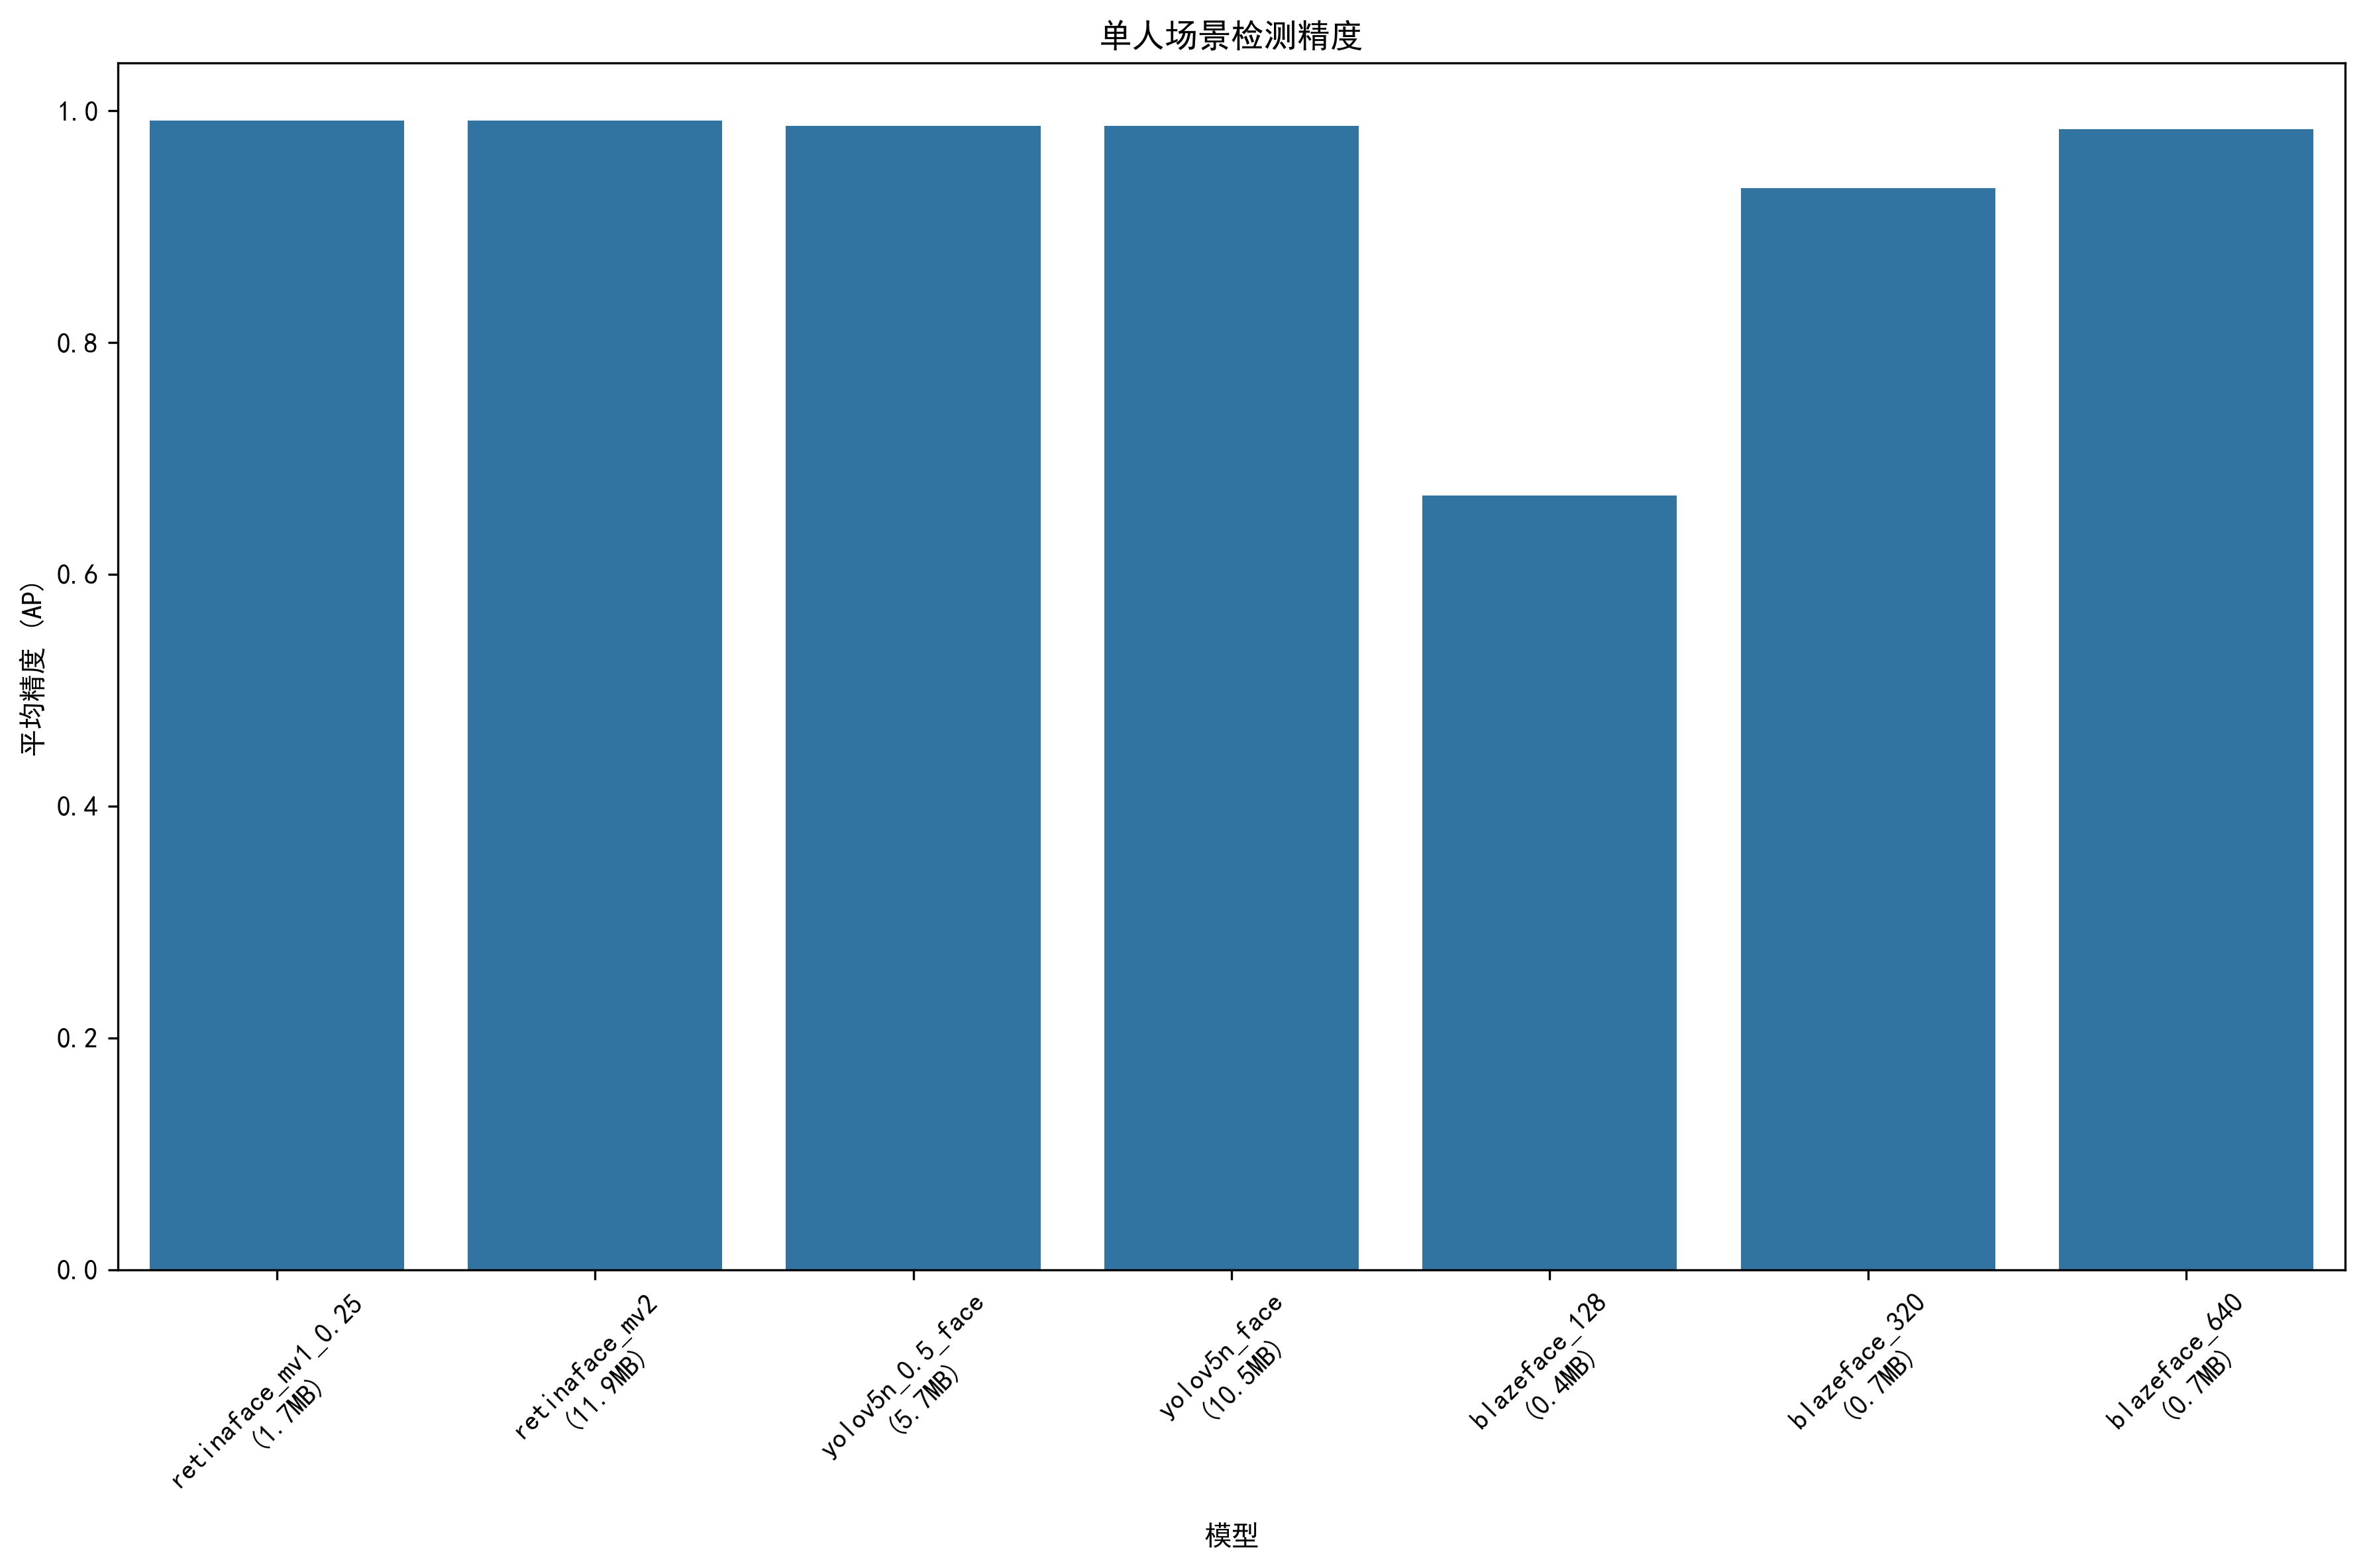
\includegraphics[width=\textwidth]{imgs/one_face_ap.png}
        \caption{单人人脸场景下的检测精度}
        \label{fig:one_face_ap}
    \end{subfigure}
    \caption{模型检测精度对比}
    \label{fig:precision_analysis}
\end{figure}

从图 \ref{fig:precision_analysis} 的检测精度分析可以得出以下结论:

\begin{enumerate}
    \item WIDER FACE 数据集上的表现:
    \begin{itemize}
        \item RetinaFace-MobileNetV2 和 YOLOv5n-face 在各难度级别上都保持较高精度
        \item BlazeFace 系列模型在困难样本上的表现较弱,但随着输入分辨率的提高,检测性能有明显提升
        \item 所有模型在简单样本上的表现都优于困难样本,这符合预期
    \end{itemize}
    
    \item light\_face 数据集上的表现:
    \begin{itemize}
        \item 除 BlazeFace-128 外,其他模型都达到了较高的检测精度(>0.93)
        \item RetinaFace 系列在单人人脸场景下表现最好,达到 0.991 的 mAP
        \item 即使是最轻量的 BlazeFace-320,在该场景下也能达到 0.932 的 mAP
    \end{itemize}
\end{enumerate}

\subsection{应用场景建议}

基于实验结果,我们针对不同应用场景提出以下模型选择建议:

\subsubsection{高精度场景}
\begin{itemize}
    \item \textbf{推荐模型}:YOLOv5n-face 或 RetinaFace-MobileNetV2
    \item \textbf{性能特点}:
    \begin{itemize}
        \item 各难度级别 AP 值均高(>0.81)
        \item 模型较大(10-12MB)
        \item 速度较慢(4-13FPS)
    \end{itemize}
    \item \textbf{适用场景}:安防监控、门禁考勤等对检测精度要求较高的场景
\end{itemize}

\subsubsection{移动端前置摄像头场景}
\begin{itemize}
    \item \textbf{推荐模型}:BlazeFace-320
    \item \textbf{性能特点}:
    \begin{itemize}
        \item 体积小(0.68MB)
        \item 速度快(46FPS)
        \item 单人人脸场景下精度达 0.932
    \end{itemize}
    \item \textbf{适用场景}:移动端实时检测场景,如相机应用、视频会议、AR 试妆等
\end{itemize}

\subsubsection{轻量级场景}
\begin{itemize}
    \item \textbf{推荐模型}:BlazeFace-128
    \item \textbf{性能特点}:
    \begin{itemize}
        \item 最小体积(0.44MB)
        \item 最快速度(70+FPS)
        \item 在 light\_face 数据集上精度尚可(0.667)
    \end{itemize}
    \item \textbf{适用场景}:资源极度受限的 IoT 设备,如智能门锁、智能手表、智能玩具等
\end{itemize}

\subsubsection{平衡场景}
\begin{itemize}
    \item \textbf{推荐模型}:YOLOv5n-0.5-face
    \item \textbf{性能特点}:
    \begin{itemize}
        \item 中等体积(5.65MB)
        \item 较快速度(22FPS)
        \item 各难度级别 AP 值均衡(0.75-0.91)
    \end{itemize}
    \item \textbf{适用场景}:需要在资源和性能间取得平衡的场景,如移动端后置摄像头应用
\end{itemize}

\clearpage

\section{总结与展望}
本研究对当前主流的轻量级人脸检测模型进行了系统性的对比分析与性能评估。通过在统一的实验环境下,对 RetinaFace、BlazeFace 和 YOLO5Face 等模型进行全面测试,我们获得了以下主要结论:

\subsection{主要结论}

\begin{enumerate}
    \item \textbf{模型性能差异显著}
    \begin{itemize}
        \item RetinaFace 和 YOLO5Face 系列在检测精度上具有明显优势,特别是在处理复杂场景时表现突出
        \item BlazeFace 系列在推理速度和模型大小上表现优异,特别适合资源受限的端侧设备
        \item YOLOv5n-0.5-face 在各项性能指标上较为均衡,为端侧部署提供了一个折中方案
    \end{itemize}

    \item \textbf{应用场景适配性}
    \begin{itemize}
        \item 不同场景对模型性能的要求存在明显差异
        \item 高精度场景(如安防监控)适合使用 YOLOv5n\_face 或 RetinaFace\_mv2
        \item 移动端前置摄像头场景推荐使用 BlazeFace\_320
        \item 资源极度受限的 IoT 设备可选择 BlazeFace\_128
        \item 需要平衡各项性能的场景可采用 YOLOv5n-0.5-face
    \end{itemize}

    \item \textbf{评估方法的有效性}
    \begin{itemize}
        \item WIDER FACE 数据集提供了标准化的性能评估基准
        \item 自建的 light\_face 数据集有效补充了实际应用场景的测试需求
        \item 统一的 ONNX 格式转换和推理流程确保了评估结果的可比性
    \end{itemize}
\end{enumerate}

\subsection{未来工作展望}

基于本研究的实验结果和分析,我们认为以下几个方向值得进一步探索:

\begin{enumerate}
    \item \textbf{模型优化方向}
    \begin{itemize}
        \item 探索新型高效特征提取网络的应用潜力,如 EfficientNet、GhostNet 等最新架构
        \item 研究知识蒸馏、模型压缩等技术在端侧人脸检测中的应用
        \item 拓展模型选择范围,评估 YuNet 等新兴轻量级人脸检测模型
        \item 探索模型量化、剪枝等优化技术对检测性能的影响
    \end{itemize}

    \item \textbf{评估体系完善}
    \begin{itemize}
        \item 构建更全面的模型鲁棒性评估方法
        \begin{itemize}
            \item 不同光照条件下的检测性能
            \item 极端姿态下的检测准确率
            \item 各类遮挡情况的处理能力
        \end{itemize}
        \item 增加更多评估维度
        \begin{itemize}
            \item 模型计算复杂度分析
            \item 内存占用情况监测
            \item 能耗水平评估
        \end{itemize}
        \item 扩充测试数据集
        \begin{itemize}
            \item 构建更具代表性的真实场景测试集
            \item 增加特定应用场景的专项测试数据
            \item 完善数据标注质量控制体系
        \end{itemize}
    \end{itemize}

    \item \textbf{工程实践优化}
    \begin{itemize}
        \item 改进评估框架的工程实现
        \begin{itemize}
            \item 提升代码的模块化程度
            \item 增强框架的可扩展性
            \item 完善自动化测试流程
        \end{itemize}
        \item 探索更多部署优化方案
        \begin{itemize}
            \item 研究不同推理框架的性能差异
            \item 优化模型在特定硬件平台上的表现
            \item 开发自适应的模型选择机制
        \end{itemize}
    \end{itemize}
\end{enumerate}

总的来说,端侧轻量级人脸检测仍是一个充满挑战和机遇的研究领域。随着移动设备和物联网技术的不断发展,对高效准确的人脸检测模型的需求将持续增长。未来的研究工作需要在模型优化、评估方法和工程实践等多个维度上持续推进,以更好地满足实际应用的需求。同时,新型网络架构、模型压缩技术和硬件加速方案的发展,也将为端侧人脸检测带来新的发展机遇。

\clearpage

% 参考文献部分
\bibliographystyle{unsrt}
\bibliography{refs}

\end{document}